\documentclass[a4paper,fleqn]{cas-dc}
\usepackage{tikz}
\usepackage{xcolor}
\usetikzlibrary{positioning, calc, backgrounds}
\usepackage{pdflscape}   % for landscape wrapping


% --- Figures & tables ---
\usepackage{graphicx}
\usepackage{booktabs}
\usepackage{multirow}
\usepackage{float}
\usepackage{subcaption}
\usepackage{mdframed}
\usepackage{booktabs}
\usepackage{caption}
\usepackage{listings}
\usepackage{longtable}
\usepackage{array}
\usepackage{pdflscape}
\usepackage{microtype}
\usepackage{arydshln}
\usepackage{enumerate}
\usepackage{tabularx}
% --- Lists/columns ---
\usepackage{multicol}
\usepackage{enumitem}
\usepackage{longtable}
% \usepackage{listings}
% --- Colors ---
\usepackage[dvipsnames,svgnames,x11names]{xcolor}

% --- Hyperlinks ---
% \usepackage[colorlinks=true,
%             linkcolor=RoyalBlue,
%             citecolor=ForestGreen,
%             urlcolor=Maroon]{hyperref}


\usepackage{array}
\usepackage{booktabs}
\usepackage{longtable}
\usepackage{xcolor}

\usepackage[most]{tcolorbox}
\usepackage{caption}
\usepackage{xcolor}

\tcbset{
    promptbox/.style={
        enhanced,
        breakable,
        colback=gray!5,
        colframe=black!60,
        boxrule=0.5pt,
        arc=0pt,
        left=6pt,
        right=6pt,
        top=6pt,
        bottom=6pt
    }
}

\newcommand{\dashedrule}{\noalign{\vskip3pt{\color{gray!40}\hrule height 0.4pt}\vskip3pt}}
\newcommand{\tabitem}{\hspace{2pt}\textbullet\hspace{5pt}}


\usepackage{ragged2e}

\newcolumntype{L}[1]{>{\RaggedRight\arraybackslash}p{#1}}

% --- Code listings ---
\usepackage{listings}
\lstset{
  basicstyle=\ttfamily\footnotesize,
  breaklines=true,
  frame=single,
  columns=fullflexible,
  keepspaces=true,
  postbreak=\mbox{\textcolor{gray}{$\hookrightarrow$}\space}
}

% --- REQUIRED for author/affiliation formatting ---
% \usepackage{authblk}

% If the frontmatter runs over more than one page
% use the longmktitle option.

%\documentclass[a4paper,fleqn,longmktitle]{cas-sc}

%\usepackage[numbers]{natbib}
%\usepackage[authoryear]{natbib}
% \usepackage[authoryear,longnamesfirst]{natbib}
\usepackage[numbers]{natbib}

%%%Author macros
\def\tsc#1{\csdef{#1}{\textsc{\lowercase{#1}}\xspace}}
\tsc{WGM}
\tsc{QE}
%%%

% Uncomment and use as if needed
%\newtheorem{theorem}{Theorem}
%\newtheorem{lemma}[theorem]{Lemma}
%\newdefinition{rmk}{Remark}
%\newproof{pf}{Proof}
%\newproof{pot}{Proof of Theorem \ref{thm}}

\begin{document}
\let\WriteBookmarks\relax
\def\floatpagepagefraction{1}
\def\textpagefraction{.001}
% Short title
\shorttitle{SLR on Angiographic Sequence Analysis}

% Short author
% \shortauthors{Khan, Filkov and Goldman}

% Main title of the paper
\title[mode = title]{A Systematic Literature Review on Methods for Angiographic Sequence Analysis}

\tnotemark[1]


% \author[1]{Nafiz Imtiaz Khan}[orcid=0000-0003-0149-6012]
% \ead{nikhan@ucdavis.edu}
% \author[1]{Vladimir Filkov}[orcid=0000-0003-0492-4393]
% \author[3]{Roger Eric Goldman}[orcid=0000-0003-0394-3744]
% \cormark[1]
% \fnmark[1]


% \credit{Conceptualization, Methodology, Software, Formal Analysis, Writing -- Original Draft}

% \affiliation[1]{organization={Department of Computer Science, University of California, Davis},
%             addressline={},
%             city={Davis},
%             postcode={95616},
%             state={CA},
%             country={USA}}
% \ead{}
% \ead[url]{}

% % Credit authorship
% \credit{Supervision, Conceptualization, Writing -- Review \& Editing}

% \ead[url]{}

% \credit{Supervision, Conceptualization, Methodology, Clinical Expertise, Writing -- Review \& Editing}

% % Address/affiliation
% \affiliation[2]{organization={Department of Radiology, School of Medicine, University of California, Davis},
%             city={Sacramento},
%             postcode={95817},
%             state={CA},
%             country={USA}}

% \cortext[1]{Corresponding author}
% \fntext[1]{}

\begin{abstract}
Cardiovascular disease remains a leading cause of mortality worldwide. Angiographic imaging serves as a cornerstone for the diagnosis and treatment of vascular disorders. Unlike static medical imaging modalities, digital subtraction angiography (DSA) and fluoroscopic acquisitions capture dynamic contrast propagation over time, providing rich spatial and temporal information that can support clinical decision-making. Recent advances in artificial intelligence (AI) and deep learning have accelerated the development of automated methods for angiographic sequence analysis; however, the literature remains fragmented across clinical domains, imaging modalities, computational tasks, and research communities. To provide a comprehensive synthesis of this rapidly evolving field, we conducted a PRISMA 2020-guided systematic literature review of AI-based angiographic sequence analysis. A structured search of PubMed/MEDLINE and Semantic Scholar identified 5,829 records, from which 194 studies satisfied all eligibility criteria and were included in the final review. We systematically analyze publication trends, imaging modalities, anatomical coverage, computational tasks, deep learning architectures, evaluation practices, reporting quality, and translational readiness. Our findings reveal substantial growth in the field since 2020, yet demonstrate that most existing approaches continue to treat angiographic sequences as collections of independent frames rather than explicitly modeling temporal dynamics. The literature is heavily concentrated in neurologic and cardiac applications, together accounting for over 70\% of included studies, with limited exploration of multi-modal learning, broader anatomical territories, and clinically grounded outcome prediction. Furthermore, considerable heterogeneity in datasets, evaluation protocols, and reporting practices constrains reproducibility and cross-study comparison. Through a synthesis of methodological limitations and future work reported across the included studies, we identify twelve major research gaps spanning data infrastructure, temporal modeling, annotation efficiency, clinical validation, explainability, multi-modal integration, privacy-preserving learning, outcome prediction, and large language model applications. Collectively, to the best of our knowledge, these findings provide the first overview of deep learning methods for angiographic sequence analysis that jointly synthesizes imaging modalities, anatomical territories, computational tasks, architectural paradigms, temporal modeling strategies, evaluation practices, and translational considerations, and establish a roadmap for the development of robust, reproducible, and clinically deployable AI systems for angiography-guided interventional procedures.

\end{abstract}


\begin{keywords}
{Angiographic Sequence Analysis \sep Digital Subtraction Angiography \sep Fluoroscopy \sep Deep Learning \sep Artificial Intelligence \sep Temporal Modeling \sep Spatio-Temporal Learning \sep Medical Image Analysis \sep Interventional Radiology \sep Cardiovascular Imaging \sep Systematic Literature Review}
\end{keywords}

\maketitle


\section{Introduction}
\label{sec:introduction}

Cardiovascular disease is one of the leading causes of death worldwide, accounting for an estimated 17.9 million deaths each year, nearly one third of all deaths~\cite{WHO2023CVD}. Catheter-based angiography is central to its diagnosis and treatment, providing real-time images of vascular anatomy and pathology during endovascular procedures~\cite{valji2011practice, kaufman2013vascular}. These procedures treat aneurysms, obstructions, malformations and traumatic injury.

Unlike most medical imaging, angiography is inherently temporal~\cite{ref89}. Digital subtraction angiography (DSA) and fluoroscopy record sequences of images that follow a contrast agent through the vessels. These dynamics carry information about vessel patency, perfusion, collateral circulation, stenosis severity and procedural outcome that no single frame contains.

The temporal nature of angiographic data also makes it hard to analyze automatically. Respiratory and cardiac motion, differences in acquisition protocol and imaging system, and varying sequence lengths all complicate automated analysis~\cite{shi2021temporal}. These challenges have drawn AI and health researchers to methods that use both the spatial and the temporal information in angiographic sequences, with the aim of more standardized and consistent readings and a lower workload for clinicians.

Angiography is also valuable for its spatial detail. Its high spatial and contrast resolution shows vessel morphology, luminal narrowing, collateral networks and device position~\cite{valji2011practice, kaufman2013vascular}, which has motivated applications ranging from vessel segmentation and landmark detection to lesion characterization, device tracking, image enhancement and procedural guidance (Section~\ref{sec:analysis}).

\subsection{AI for Angiographic Sequence Analysis}
Deep learning has changed medical image analysis, from detection and segmentation to reconstruction and decision support~\cite{Litjens2017,Topol2019}. Convolutional, encoder--decoder, Transformer and hybrid models perform well on many tasks traditionally done by clinical experts~\cite{Litjens2017,Shen2017}. In angiography, researchers have applied these models to enhancement, vessel segmentation, motion correction, device tracking, landmark detection, outcome prediction and procedural guidance~\cite{ref99, ref100}, and many of these tasks involve information that changes over time.

This literature is fragmented. It is spread across cardiology, radiology, surgery, computer vision, biomedical engineering and machine learning venues, with different datasets, evaluation protocols and metrics. In particular, it is unclear how temporal information is used across tasks: whether frames are processed independently, combined by fixed operations such as stacking or registration, or modeled with learned sequence architectures. Whether learned temporal models outperform frame-independent ones cannot be settled across studies with different datasets and metrics; it requires controlled comparisons on shared benchmarks.

\subsection{The Need for a Systematic Review}
Earlier surveys cover deep learning in medical imaging at large~\cite{Litjens2017,Shen2017} or vascular imaging in general~\cite{Moccia2018}, without focusing on angiographic sequences. Reviews of AI in interventional radiology~\cite{Iezzi2019,Gurgitano2021,Mukhtar2025} describe its role in planning, guidance, workflow and interpretation, and note limited data, little external validation, heterogeneous evaluation and regulatory barriers, but they focus on clinical use rather than on the methods that analyze image sequences.

To our knowledge, no review has examined AI methods that operate on X-ray angiographic sequences while also covering modalities, territories, tasks, architectures, temporal modeling, evaluation and reporting. Clinical translation of these methods depends on rigorous validation, transparent reporting and evidence that models generalize across institutions, vendors and patients~\cite{Tejani2024,collins2024tripod+}, so these aspects need to be assessed alongside the methods themselves.

\subsection{Objectives}
\label{sec:intro-objectives}

This review has four objectives:

\begin{enumerate}[label=\textbf{O\arabic*.}, leftmargin=*, itemsep=4pt]
\item \textbf{Characterize the field:} catalog AI methods, predominantly deep learning, applied to DSA and fluoroscopic sequences across clinical and technical tasks.
\item \textbf{Examine temporal modeling:} identify how temporal information is represented across architectures and applications.
\item \textbf{Assess evidence quality:} review datasets, evaluation practices, reporting and reproducibility.
\item \textbf{Identify research gaps:} set out directions toward reliable, clinically deployable methods.
\end{enumerate}

The review is written for clinicians who use angiography, for medical imaging and machine learning researchers, and for developers of clinical AI systems.

\section{Methodology}
\subsection{Search Strategy}
This systematic review was conducted in accordance with the Preferred Reporting Items for Systematic Reviews and Meta-Analyses 2020 (PRISMA 2020) guidelines~\cite{Page2021PRISMA}. As the primary objective of this review is to characterize AI methods that operate on angiographic image sequences, the search strategy was designed to jointly capture both the imaging modality and the computational methodology.

A structured Boolean search was executed across PubMed/MEDLINE \cite{white2020pubmed} and Semantic Scholar \cite{fricke2018semantic}. These databases were selected to provide complementary coverage of both clinical and technical literature, which reflects the interdisciplinary nature of angiographic image analysis research. No study-type filters were applied during database retrieval in order to maximize recall and avoid prematurely excluding potentially relevant methodological contributions. Instead, study eligibility was determined during the screening process.

The search spans publications published between \textit{January 1, 2000} and \textit{15 May 2026}. The year 2000 was selected as a practical lower bound because modern digital angiographic workflows and contemporary machine learning approaches largely emerged after this period.

To capture studies at the intersection of angiographic imaging and AI, the search query was organized into two Boolean components.

\medskip
\noindent\textbf{Block 1 --- Imaging modality}
\begin{quote}
\small\texttt{(angiograph* OR fluoroscopy* OR ``digital subtraction angiography'' OR DSA)}
\end{quote}

\noindent\textbf{AND}

\noindent\textbf{Block 2 --- Computational methodology}
\begin{quote}
\small\texttt{(`deep learning'' OR `machine learning'' OR CNN OR transformer OR ``artificial intelligence'' OR AI)}
\end{quote}
\medskip

% The initial search yielded 5{,}829 records, including 4{,}071 from PubMed/MEDLINE and 1{,}758 from Semantic Scholar. Duplicate records were removed, which resuls in the exclusion of 765 duplicates and leaving 5{,}064 unique records. An additional 29 records lacking retrievable titles or abstracts were excluded prior to screening, yielding 5{,}035 records for title and abstract assessment.



\subsection{Eligibility Criteria}
\label{sec:eligibility}

Eligibility criteria were defined \emph{a priori} in accordance with PRISMA 2020 recommendations and are summarized in Table~\ref{tab:criteria}. 

To be included, a study was required to satisfy four inclusion criteria. First, the study had to analyze DSA or fluoroscopic image sequences containing explicit temporal information. Second, it had to address at least one computational processing task relevant to angiographic analysis, which includes image enhancement, denoising, background subtraction, motion correction, registration, vessel segmentation, object detection, classification, temporal sequence modeling, or outcome prediction. Third, the proposed methodology had to be described with sufficient technical detail to identify the principal processing pipeline and model architecture. Fourth, the study was required to report quantitative evaluation results using a defined validation strategy.

Studies were excluded if they focused exclusively on non-angiographic imaging modalities, operated solely on static images without sequence-level analysis, lacked an original computational contribution, were available only as abstracts or posters without sufficient methodological detail, or were not available in English. Eligibility criteria were applied sequentially during title--abstract screening and subsequently re-evaluated during full-text assessment.


\subsection{LLM-Assisted Screening Pipeline}
\label{sec:llm-pipeline}

Given the large volume of retrieved records, an LLM-assisted screening workflow was developed to support the systematic review process while maintaining explicit adherence to predefined eligibility criteria. The objective of the pipeline was not to replace human judgment but rather to provide a scalable and reproducible mechanism for applying the inclusion and exclusion criteria consistently across thousands of candidate records. All inference was performed locally using the Ollama framework \cite{marcondes2025using}, which enabled complete control over model execution, eliminated dependence on external services, and ensured reproducibility of the screening process.

The screening workflow consisted of two sequential stages corresponding to the title--abstract screening and full-text review phases of the systematic review. During the first stage, candidate records were evaluated using a structured two-gate screening architecture. The first gate assessed the four inclusion criteria (I1--I4), requiring all criteria to be satisfied before a study could advance. Records passing the inclusion gate were subsequently evaluated against the exclusion criteria (E1--E5). Any study triggering one or more exclusion criteria was removed from further consideration. This design mirrors the sequential decision-making process, which is commonly employed during manual systematic reviews and provides explicit traceability regarding the criterion responsible for each exclusion decision.

\subsubsection{Title-Abstract Eligibility Assessment}
\label{sec:title-abstract-sceening}

For each record, the model was provided with the article title and abstract and instructed to generate a structured JSON response containing: (i) an inclusion or exclusion decision, (ii) the eligibility criteria that were satisfied or violated, (iii) a concise justification for the decision, and (iv) an uncertainty flag indicating whether insufficient information was available for a confident assessment. To maximize determinism and reduce response variability, model temperature was fixed at zero. Additional safeguards included automatic retry mechanisms, JSON schema validation, response repair procedures for malformed outputs, and context-length controls for unusually long abstracts. Records classified as uncertain were automatically flagged for human review.

Because screening decisions directly influence the composition of the final review corpus, a manual validation procedure was conducted to assess the reliability of the LLM-assisted workflow. A random sample of 100 records was independently reviewed by a human evaluator (NIK) using the same inclusion and exclusion criteria applied by the automated pipeline. The evaluator assessed each article without access to the model-generated decision and subsequently compared the resulting judgments against the LLM outputs. Disagreements were examined manually to identify potential failure modes and verify the suitability of the screening pipeline for large-scale literature assessment. This validation step provided an additional layer of quality assurance and reduced the likelihood of systematic screening errors.

%Studies that advanced beyond title--abstract screening proceeded to a full-text analysis stage. Full manuscripts were converted into machine-readable Markdown representations and processed using GPT-OSS:20B \cite{agarwal2025gpt} deployed locally through Ollama \cite{marcondes2025using}. GPT-OSS:20B was selected because it provides strong reasoning and structured information extraction capabilities while remaining computationally practical for large-scale document analysis. Recent evaluations have demonstrated that GPT-OSS models achieve performance competitive with substantially larger models on information extraction, scientific document understanding, and structured reasoning tasks, making them well suited for systematic review workflows \cite{agarwal2025gpt, OpenAI2025GPTOSS}. The model was instructed to extract a comprehensive set of bibliographic, methodological, evaluative, and translational characteristics according to a predefined JSON schema. Extracted fields included imaging modalities, anatomical territories, dataset characteristics, computational tasks, architectural designs, temporal modeling strategies, evaluation metrics, validation methodologies, reproducibility indicators, and clinical deployment considerations.

%To ensure transparency and reproducibility, the prompts are provided in Appendix A.


\subsubsection{Full-Text Eligibility Assessment and Structured Data Extraction}
\label{sec:full-text-screening}

Studies advancing beyond title--abstract screening underwent full-text eligibility assessment and structured information extraction. Full manuscripts were converted into machine-readable Markdown representations and processed using a second LLM-based extraction pipeline.

This stage employed GPT-OSS:20B \cite{agarwal2025gpt}, an open-weight large language model deployed locally through Ollama. GPT-OSS:20B was selected because it provides strong reasoning and information extraction performance while remaining computationally practical for large-scale full-text analysis. Recent benchmarking studies have demonstrated that GPT-OSS models achieve performance comparable to substantially larger proprietary and open-source models across a range of structured extraction and scientific document understanding tasks, making them well-suited for systematic review workflows.

For each article, the model was provided with the full manuscript text and instructed to extract information according to a predefined JSON schema developed specifically for angiographic sequence analysis. Extracted fields included bibliographic metadata, imaging modality, anatomical territory, dataset characteristics, annotation procedures, computational tasks, model architectures, temporal modeling strategies, evaluation metrics, validation designs, reproducibility indicators, clinical validation characteristics, limitations, and future research directions.

To maximize extraction consistency, model outputs were constrained to structured JSON representations and validated automatically. Malformed outputs triggered automated repair procedures and re-evaluation. Full-text inputs exceeding the model context budget were truncated using a predefined maximum character limit while preserving the article metadata and primary methodological content.

The resulting structured database served as the foundation for all subsequent quantitative analyses presented in Section~\ref{sec:results}. The complete extraction schema, prompts, and implementation details are provided in Appendix~X.

\subsection{Statistical Analysis}
\label{sec:stats-methods}
Statistical analyses were primarily descriptive in nature and were designed to characterize methodological, reporting, and performance trends across the included studies. Frequencies, percentages, and summary distributions were computed for publication characteristics, imaging modalities, anatomical territories, computational tasks, model architectures, and reporting attributes. Reporting-quality assessments based on the CLAIM 2024 framework were summarized as adherence proportions, with corresponding 95\% confidence intervals estimated using the Wilson score method. Comparative analyses between publication cohorts were performed using differences in observed proportions, with studies split into a pre-2025 cohort ($\leq 2024$) and a post-2025 cohort ($\geq 2025$) to evaluate temporal changes in reporting adherence following the release of CLAIM 2024. For each reporting item, the difference between cohort proportions ($\Delta$) was computed, and changes exceeding 2 percentage points were flagged as directionally meaningful. Reported performance metrics extracted from the literature were aggregated and examined using histograms and kernel density estimation (KDE) to visualize distributional patterns across metric families. Given the substantial heterogeneity in datasets, validation protocols, and evaluation metrics among studies, no formal meta-analysis or pooled effect-size estimation was performed. All statistical analyses and visualizations were conducted using Python.
% \subsection{Screening and Selection Process}
% \label{sec:screening}

% Screening was conducted using a two-stage process, shown in Figure~\ref{fig:prisma}. The two-stage design was adopted to balance broad initial coverage with detailed full-text verification, allowing potentially relevant studies to be retained until sufficient methodological information became available for eligibility assessment.

% \textbf{Stage 1 --- Title and abstract screening.}

% All records produced from the structured Boolean search were evaluated using the LLM-assisted screening pipeline described in Section~\ref{sec:llm-pipeline}. For each record, the system generated an INCLUDE or EXCLUDE decision accompanied by a structured rationale explicitly referencing the eligibility criteria. To assess screening reliability, a random subset (n=100) of decisions was manually reviewed by a human evaluator. 

% % Human evaluator independently looked for the decisions (include/exclude) for that random set of articles, and a 

% Following title and abstract screening, 353 records satisfied all inclusion criteria and advanced to full-text review. The remaining 4{,}682 records were excluded. The most common exclusion reason was incorrect imaging modality (E1; $n=114$), followed by the absence of temporal sequence analysis (E2; $n=29$) and non-English publication (E5; $n=1$).

% \textbf{Stage 2 --- Full-text eligibility assessment.}

% Full texts were sought for all 353 studies identified during Stage~1. Fifteen reports could not be retrieved, leaving 338 studies available for detailed eligibility assessment. Each study was evaluated against the complete inclusion and exclusion criteria using the full manuscript.

% During full-text review, 144 studies were excluded after closer examination of their methodology, datasets, or evaluation procedures. The remaining \textbf{194 studies} satisfied all eligibility requirements and were included in the final review corpus. Reasons for exclusion at this stage were recorded in accordance with PRISMA 2020 reporting guidelines and are summarized in Figure~\ref{fig:prisma}.

% % \medskip
% % \noindent\textbf{PRISMA flow sFummary.}

% In total, 5{,}829 records were identified across the two databases. After removal of duplicates and records lacking sufficient bibliographic information, 5{,}035 records underwent title and abstract screening. Of these, 353 advanced to full-text review, 338 full texts were successfully retrieved, and 194 studies ultimately met all eligibility criteria and were included in the systematic review.



\section{Results}
\label{sec:analysis}
\label{sec:results}
We first report study selection and the validation of screening and extraction, then the characteristics of the 120 included studies: publication trends, modalities and territories, tasks and architectures, temporal modeling, venues, reported performance and reporting quality.

\subsection{Study Selection and Review Corpus}
The search identified 5,829 records (PubMed/\allowbreak MEDLINE 4,071; Semantic Scholar 1,758). After removing 765 duplicates, we screened 5,064 records (Figure~\ref{fig:prisma}). The LLM labelled 134 as eligible and excluded 4,930: 4,831 failed at least one inclusion criterion and 99 met an exclusion criterion (E1: 3, E2: 95, E3: 1). Cochran's formula set the validation sample at 357 of the 4,930 exclusions, so the reviewers screened 491 records.

The two reviewers agreed on 487 of the 491 records (99.2\%; Cohen's $\kappa=0.978$, 95\% CI 0.957--0.999). Each reviewer included two records the other excluded; in all four cases the consensus followed the interventional radiologist. Against this gold standard, the pipeline was correct for 120 of its 134 INCLUDE decisions (89.6\%; 95\% Wilson CI 83.2--93.7\%) and for 355 of the 357 sampled EXCLUDE decisions (99.4\%; 98.0--99.8\%). Weighted by stratum size, overall agreement was 99.2\%, and precision, recall and F1 for the INCLUDE class were 0.90, 0.81 and 0.85 ($\kappa=0.85$). The recall estimate rests on two missed studies, both of which failed criterion I2, and is imprecise (Section~\ref{sec:limitations}).

Following the gold standard, we excluded 14 LLM-eligible records and added the 2 eligible records found among the exclusions, giving 122 eligible studies; Figure~\ref{fig:prisma} therefore lists 4,829 rather than 4,831 LLM inclusion failures. Full text could not be retrieved for 2 of them (R4468, R4475), so the review corpus comprises 120 studies. Three are earlier versions (preprint or conference paper) of another included study and are counted separately. All 491 screening decisions are listed in Supplementary Table~S1.

The extraction audit covered 6 of the 120 studies (5\%) and 444 values: per study, 18 study-level fields, the status of the 12 research gaps and the 44 CLAIM 2024 items. The reviewer judged 431 values correct (97.1\%; 95.1--98.3\%), 13 incorrect and none unclear. All errors were interpretive (the task labels of one study, gap statuses and individual CLAIM items); descriptive fields such as modality, territory, cohort size, temporal category and validation design were correct in all six studies. Per-gap counts and item-level CLAIM percentages should therefore be read as approximate.

\begin{figure*}[htbp]
  \centering
  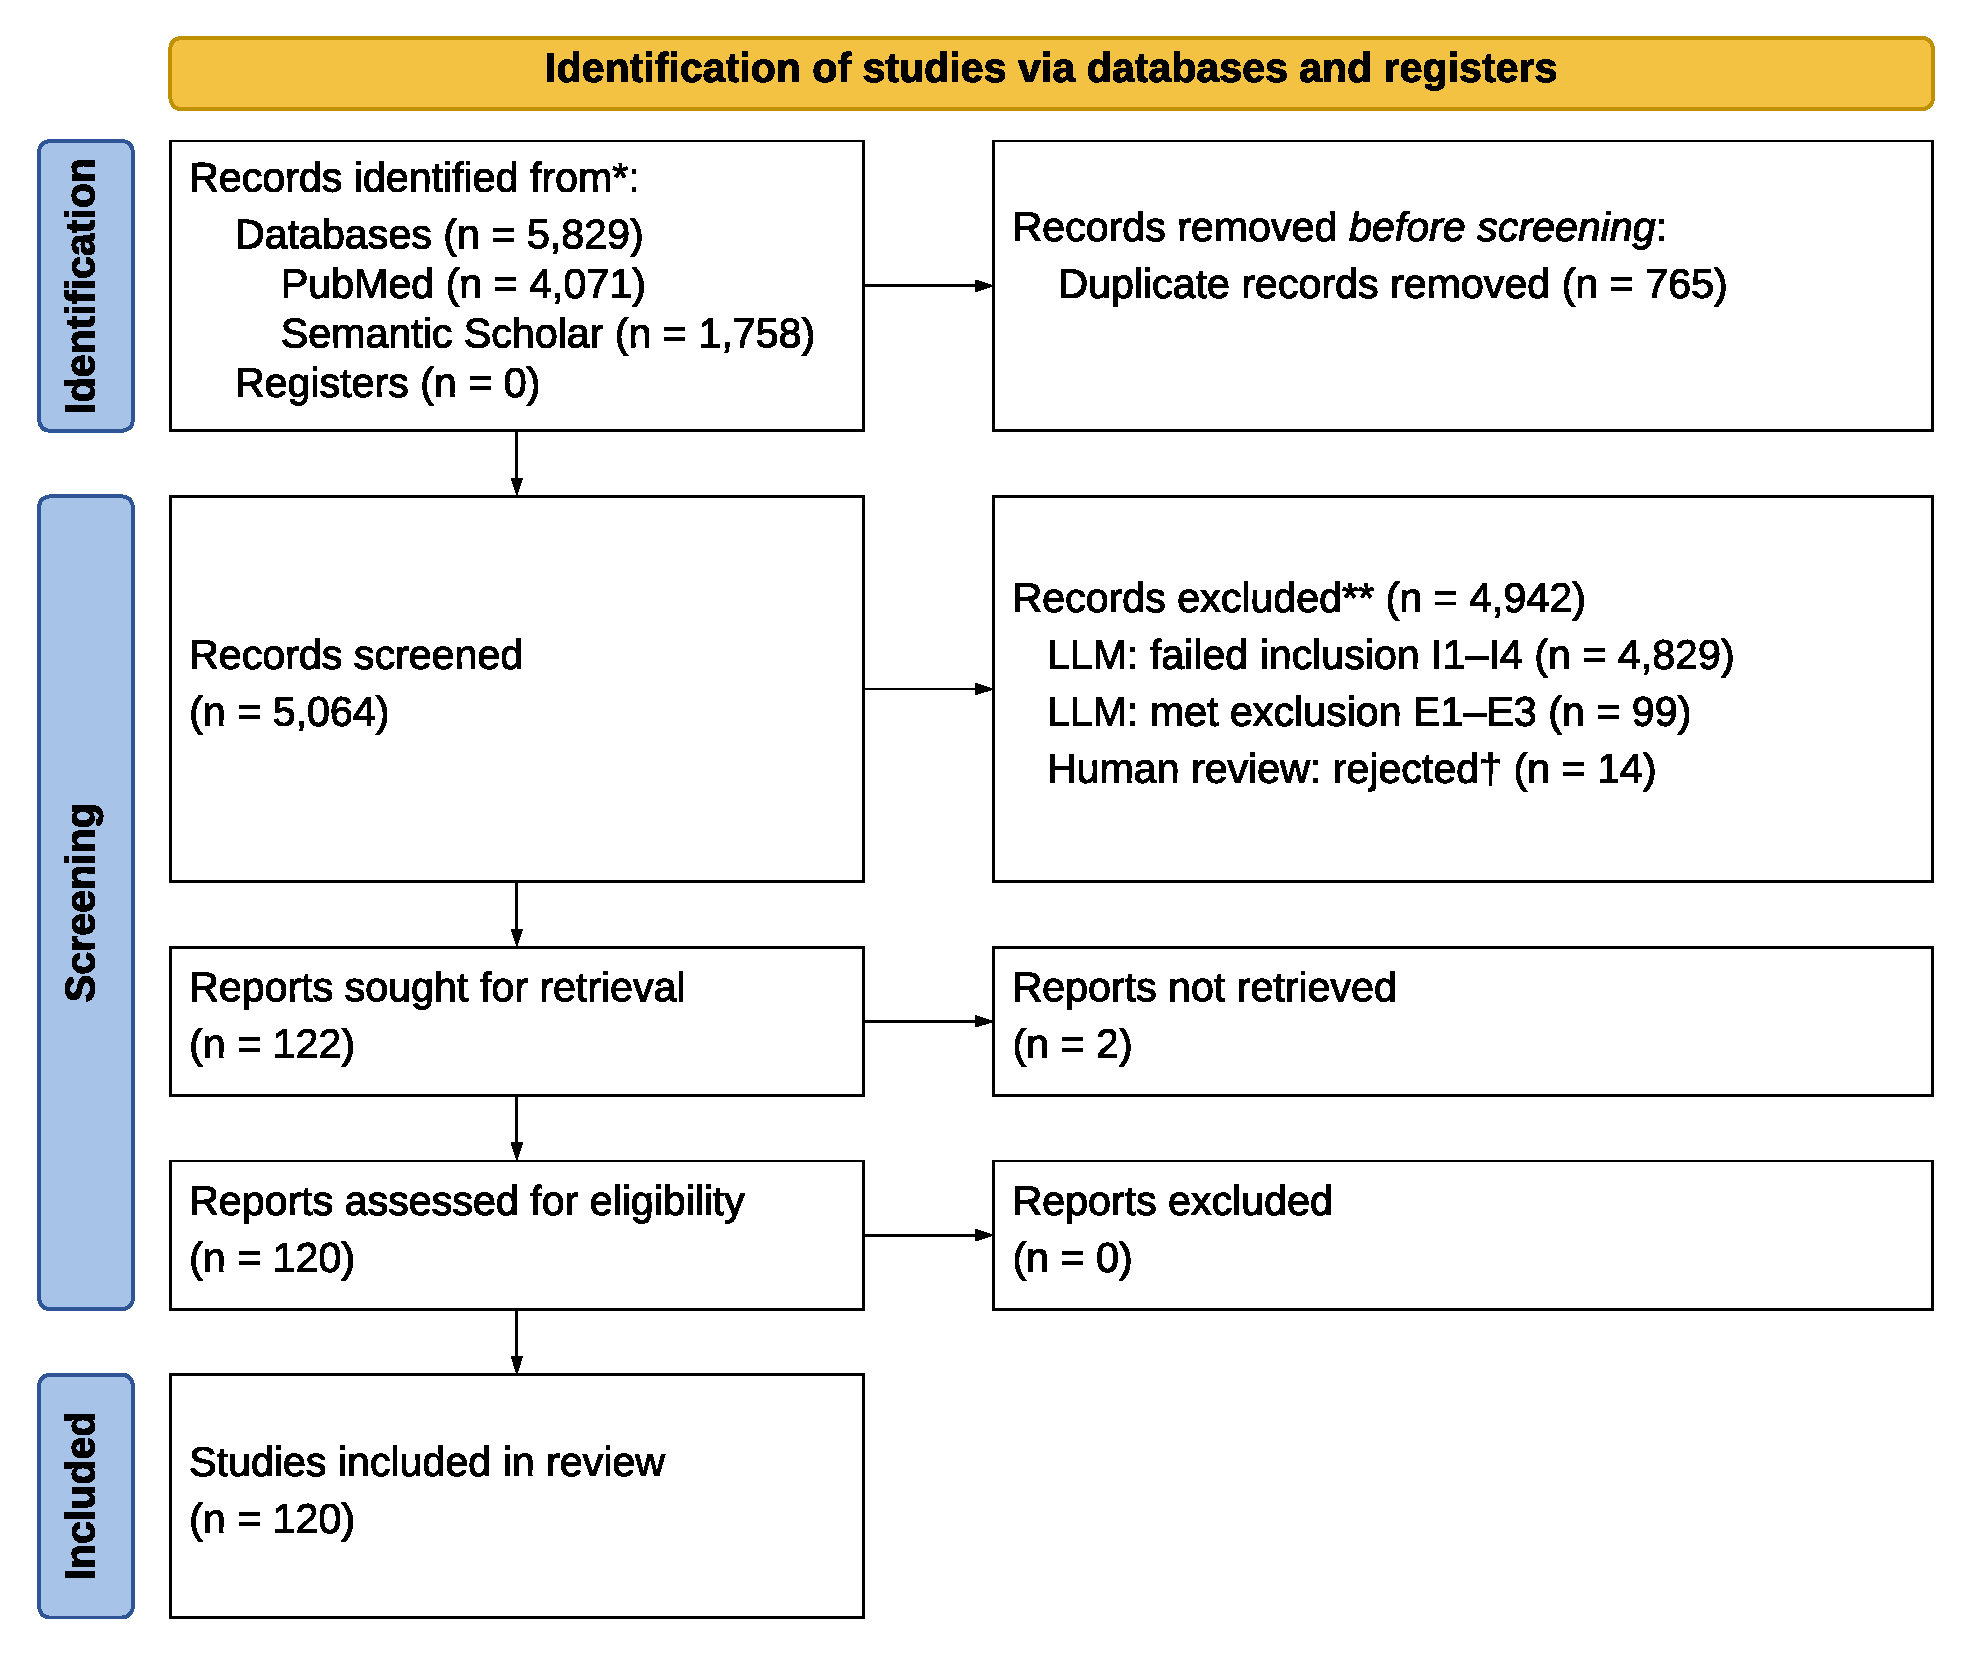
\includegraphics[width=\textwidth]{figs/prisma.pdf}
  \caption{PRISMA 2020 flow diagram summarizing the study identification, screening, eligibility assessment, and inclusion process used in this systematic review}
  \label{fig:prisma}
\end{figure*}



\subsection{Publication Trends}
\label{subsec:trends}
\begin{figure}[]
\centering
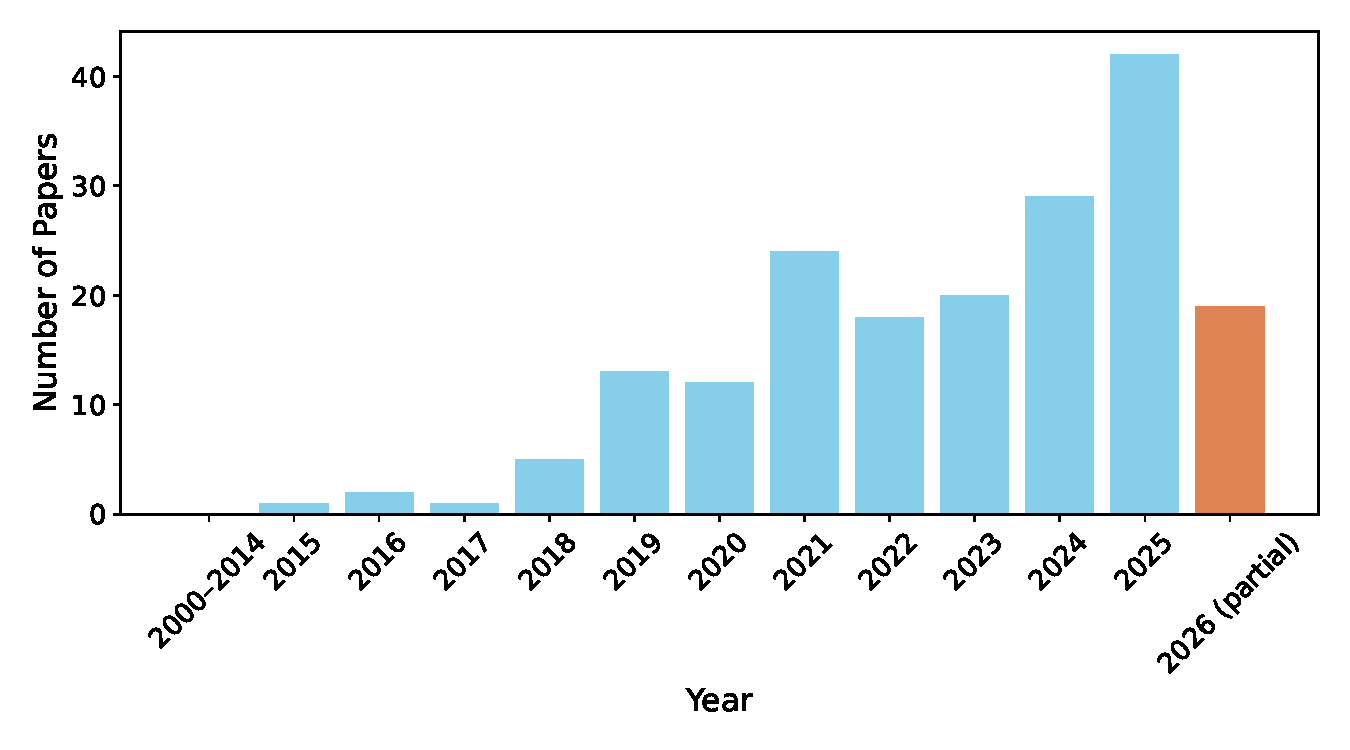
\includegraphics[width=1\linewidth]{figs/temporal_trends.pdf}
\caption{Included studies by publication year. The 2026 bar covers a partial year.}
\label{fig:temporal_trends}
\end{figure}

No included study predates 2018, and only five appeared in 2018--2019 (Figure~\ref{fig:temporal_trends}). Output rose sharply after 2020 and stayed high through 2025; the partial year 2026 already exceeds several earlier full years. Transformer-based temporal models came late: all ten in the corpus were published from 2023 onward.

\vspace{0.25cm}
\begin{mdframed}[linewidth=0.5pt, linecolor=black, backgroundcolor=blue!10]
\textbf{Finding 1.} The field is young and still growing: 78\% of studies (94/120) were published from 2022 to 2026.
\end{mdframed}
\vspace{0.25cm}

\subsection{Imaging Modalities and Anatomical Coverage}
\label{subsec:modality_anatomy}
\begin{figure}[]
\centering
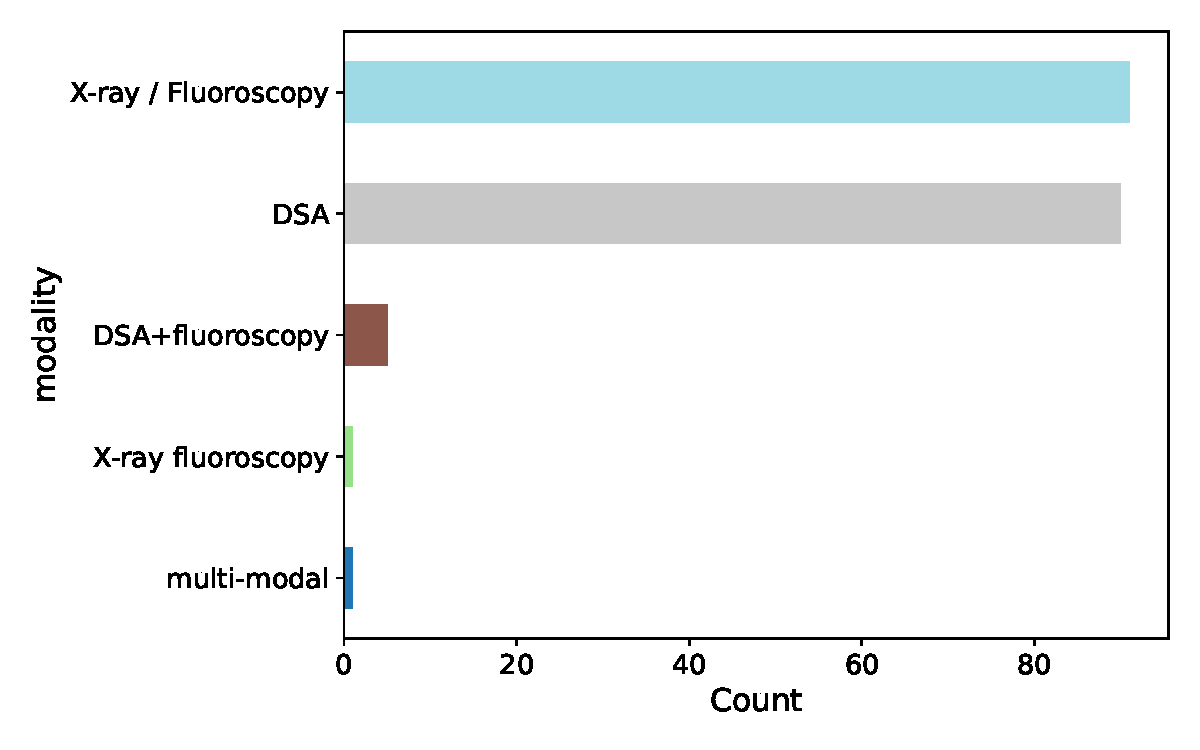
\includegraphics[width=1\linewidth]{figs/modality_distribution.pdf}
\caption{Imaging modality distribution across included studies.}
\label{fig:modality_distribution}
\end{figure}
\begin{figure}[]
\centering
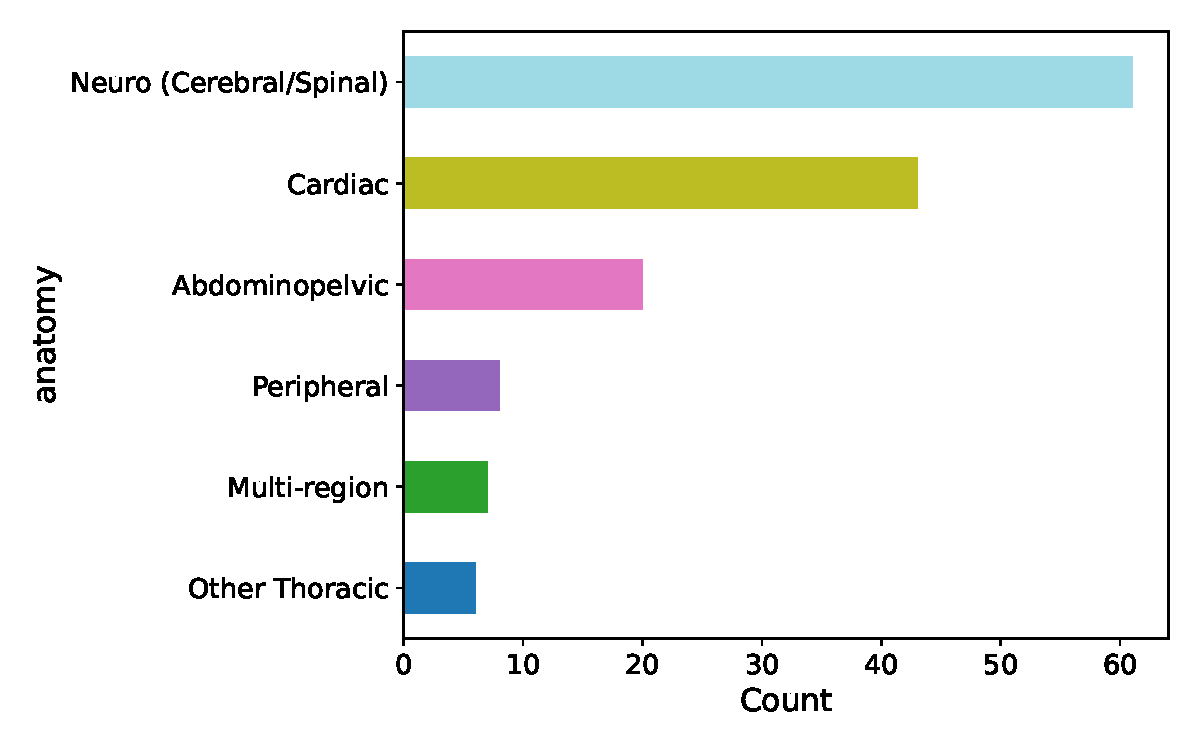
\includegraphics[width=1\linewidth]{figs/anatomy_distribution.pdf}
\caption{Territory distribution across included studies. The Neurologic category includes cerebral and spinal vascular territories.}
\label{fig:anatomy_distribution}
\end{figure}

DSA and X-ray/fluoroscopy are almost equally common (47\% and 48\% of studies; Figure~\ref{fig:modality_distribution}), but only 5 studies (4\%) use both. Cardiac (47\%) and neurologic (41\%) applications make up nearly 90\% of the corpus, while abdominopelvic, peripheral and other thoracic territories are rare (Figure~\ref{fig:anatomy_distribution}). Whether models trained on coronary or cerebral angiography transfer to other vascular beds is rarely tested.

\vspace{0.25cm}
\begin{mdframed}[linewidth=0.5pt, linecolor=black, backgroundcolor=blue!10]
\textbf{Finding 2.} Studies use DSA or X-ray/\allowbreak fluoroscopy in nearly equal numbers but almost never both, and nearly 90\% address cardiac or neurologic territories.
\end{mdframed}
\vspace{0.25cm}

\subsection{Computational Tasks and Architectures}
\label{subsec:tasks_architectures}
\begin{figure}[]
\centering
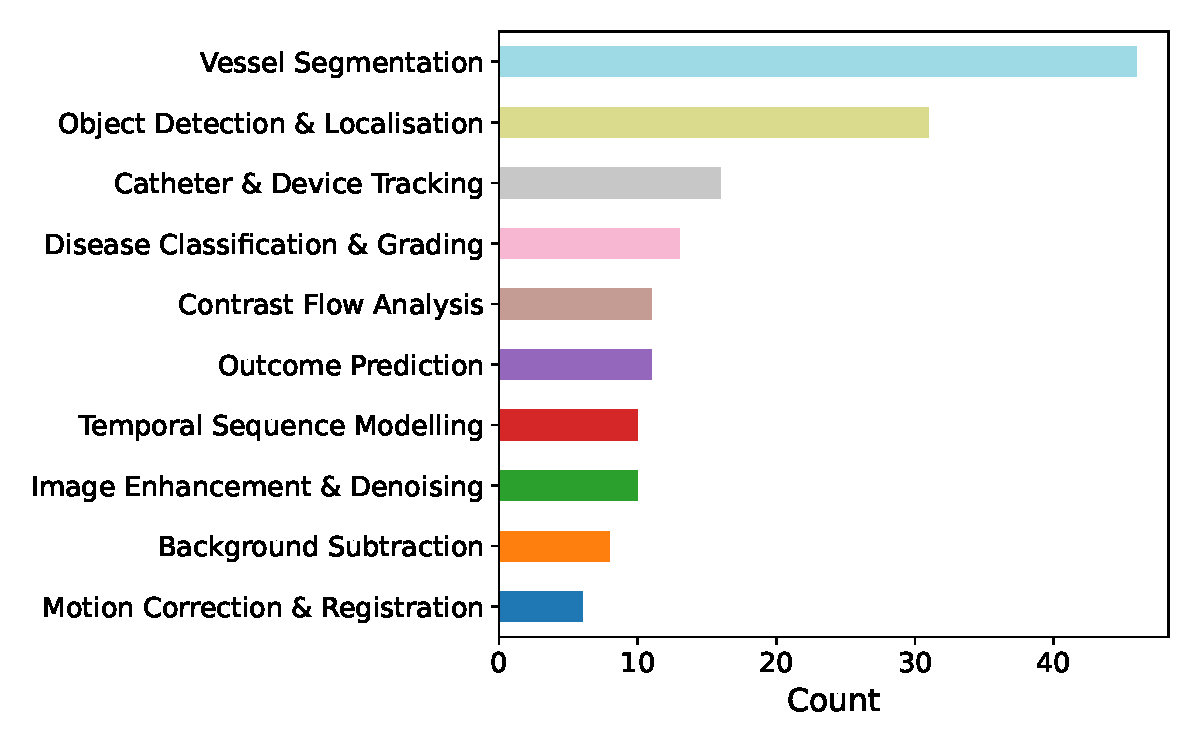
\includegraphics[width=1\linewidth]{figs/task_distribution.pdf}
\caption{Distribution of primary computational tasks across included studies.}
\label{fig:task_distribution}
\end{figure}

Disease classification and grading is the most common primary task (31 of 120 studies), followed by object detection and localization (18) and vessel segmentation (15) (Figure~\ref{fig:task_distribution}). Architectures follow the task (Table~\ref{tab:task_architecture_clean}): 14 of the 15 segmentation studies use encoder--decoder models, mostly U-Net variants; detection studies use YOLO, DETR and R-CNN detectors on ResNet backbones; classification relies on ResNet-style CNNs, with Transformers increasingly added. Most architectures are adapted from natural-image computer vision rather than designed for angiography.

Tasks whose output is itself temporal remain rare: temporal sequence modeling (6 studies) and contrast flow analysis (9). Many spatial tasks, such as segmentation, detection and classification, use several frames only to stabilize a per-frame prediction (Section~\ref{subsec:temporal_taxonomy}).

\subsubsection{Task Category Overlap}
\label{subsec:task_dendrogram}
\begin{figure}[]
\centering
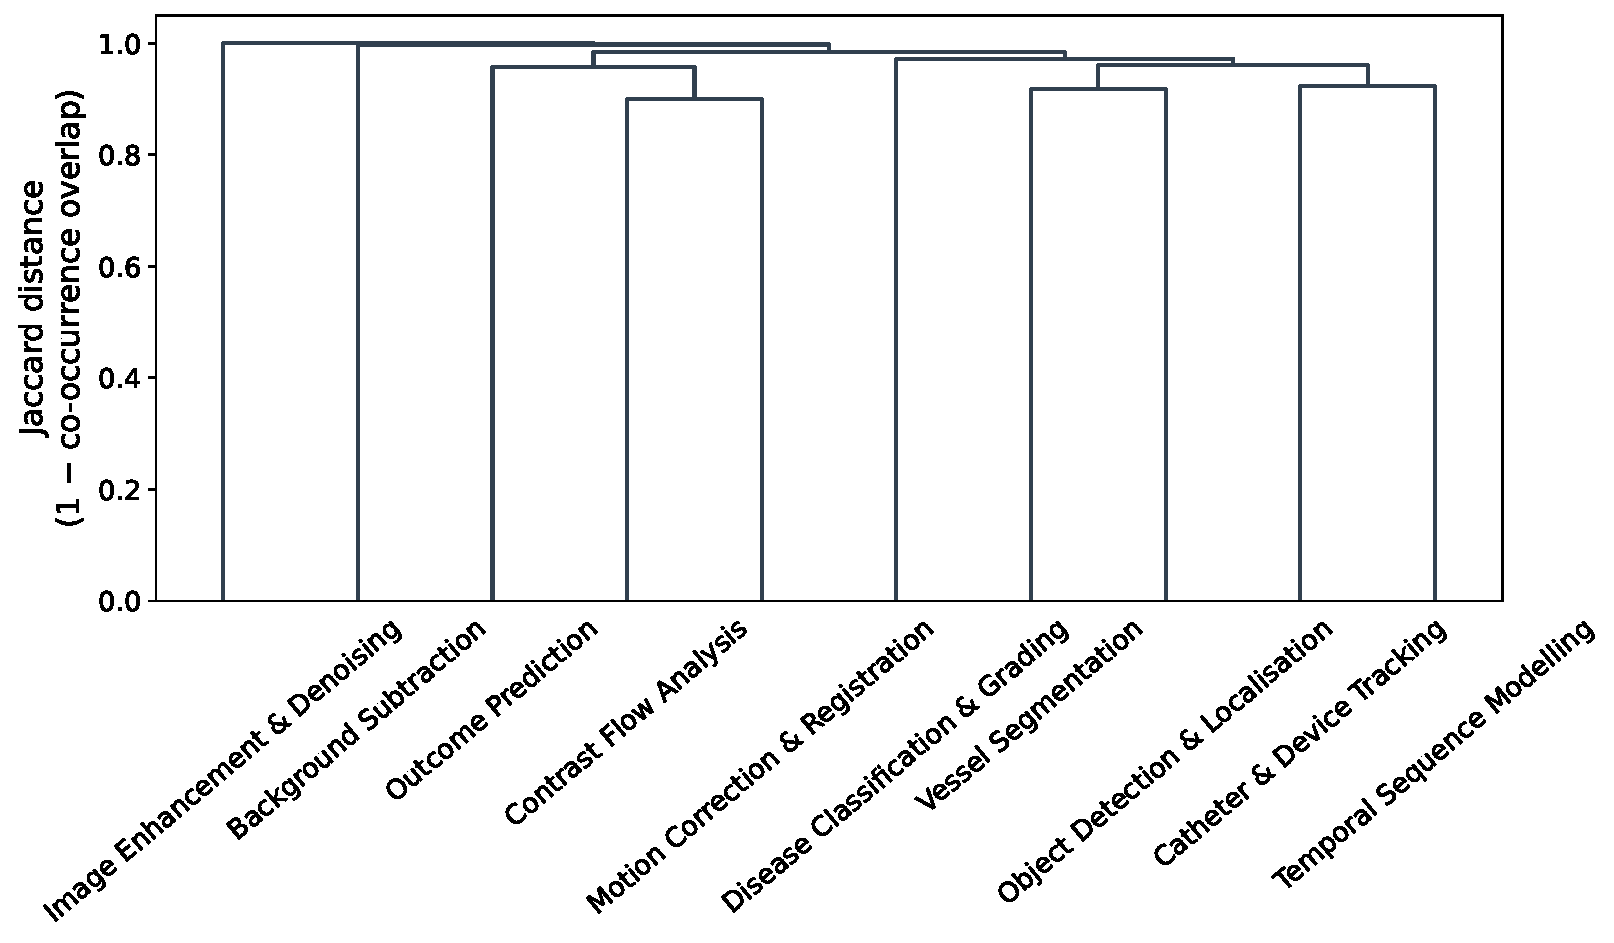
\includegraphics[width=1\linewidth]{figs/task_dendrogram.pdf}
\caption{Average-linkage (UPGMA) clustering of the ten primary task categories by Tanimoto distance between the sets of studies in each category. Merges further left mean more frequent co-occurrence. All merges fall between 0.75 and 1.00, so the axis is zoomed to that range; the two lowest sub-clusters are colored.}
\label{fig:task_dendrogram}
\end{figure}

Most task pairs merge near the maximum Tanimoto distance, so the ten categories are largely distinct (Figure~\ref{fig:task_dendrogram}). Three pairs merge earlier and are the natural candidates for a coarser taxonomy: contrast flow analysis with outcome prediction (flow measurements used as outcome predictors), classification with detection (lesions detected, then graded), and temporal sequence modeling with segmentation (vessels separated by filling phase). Image enhancement with device tracking, and motion correction with background subtraction, join the rest of the tree last.

\subsubsection{Temporal Modeling}
\label{subsec:temporal_taxonomy}
\renewcommand{\arraystretch}{1.25}
\begin{table*}[ht]
\centering
\caption{Operational taxonomy of temporal-modeling strategies, derived from the
\texttt{method.temporal\_modelling} flag and \texttt{method.temporal\_mechanism}
free-text field recorded during full-text extraction, classified via a
deterministic keyword-based rule set. N and \% are computed over the 206
records that reached full-text extraction.}
\label{tab:temporal_taxonomy}
\begin{tabularx}{\textwidth}{@{}l X r r@{}}
\toprule
\textbf{Category} & \textbf{Operational Definition} & \textbf{N} & \textbf{\%} \\
\midrule
No Temporal Use
  & Each frame (or a spatially/temporally pooled representation) is processed
    independently, with no explicit mechanism linking information across frames.
  & 129 & 62.6\% \\
\hdashline
Frame Aggregation
  & Multiple frames are combined via simple, non-learned operations (channel
    stacking, concatenation, frame differencing) before a standard 2D model.
  & 9 & 4.4\% \\
\hdashline
Optical Flow / Registration
  & Explicit frame-to-frame motion estimation, registration, or classical
    tracking/association (e.g., optical flow, particle filters,
    cross-correlation).
  & 12 & 5.8\% \\
\hdashline
RNN / LSTM / GRU
  & Recurrent architectures (LSTM, GRU, ConvLSTM, recurrent residual modules)
    propagate a hidden state across the sequence.
  & 12 & 5.8\% \\
\hdashline
3D CNN / Video Model
  & 3D or spatiotemporal convolutions, or video-/sequence-level representation
    learning, treating the sequence as a joint spatiotemporal volume.
  & 15 & 7.3\% \\
\hdashline
Transformer / State-Space
  & Self-attention or state-space mechanisms modeling long-range dependencies
    across frames.
  & 9 & 4.4\% \\
\hdashline
Hemodynamic / Physics-Informed
  & Explicit physiological or physics-based temporal modeling (reduced-order
    flow models, hemodynamic priors, physiologic signal filtering).
  & 6 & 2.9\% \\
\midrule
Not reported in extraction
  & Full-text extraction did not yield a determinable temporal-modeling
    classification for this record.
  & 14 & 6.8\% \\
\midrule
\textbf{Total} & & \textbf{206} & \textbf{100.0\%} \\
\bottomrule
\end{tabularx}
\end{table*}


Of the 120 studies, 97 (80.8\%) use an explicit mechanism that links frames, 21 (17.5\%) process frames independently, and 2 (1.7\%) do not state how frames enter the model (Table~\ref{tab:temporal_taxonomy}). The high rate partly reflects our requirement for sequence data (I2). The most common strategies are 3D/video convolution (20 studies), optical flow or registration (19) and recurrent networks (18), followed by frame aggregation (15) and hemodynamic or physics-based models (15). Transformer or state-space models are the least common (10, 8.3\%).

\renewcommand{\arraystretch}{1.2}
\begin{table*}[pos=ht]
\centering
\caption{Share of studies using explicit temporal modeling (any category in Table~\ref{tab:temporal_taxonomy} except ``No Temporal Use'') by primary task, modality and territory. Rows with fewer than 5 studies are omitted: Background Subtraction (4); Other task (1); Other modality (1); Peripheral (1); Other Thoracic (incl. aortic) (2); Multi-region (1); Not reported (1).}
\label{tab:temporal_crosstab}
\begin{tabularx}{\textwidth}{@{}X r r@{}}
\toprule
\textbf{Dimension} & \textbf{N} & \textbf{Temporal-Use Rate} \\
\midrule
\multicolumn{3}{@{}l}{\textit{By Primary Task}} \\
\dashedrule
Temporal Sequence Modelling & 6 & 100\% \\
Contrast Flow Analysis & 8 & 100\% \\
Outcome Prediction & 9 & 89\% \\
Image Enhancement \& Denoising & 9 & 89\% \\
Vessel Segmentation & 15 & 87\% \\
Disease Classification \& Grading & 29 & 83\% \\
Motion Correction \& Registration & 9 & 78\% \\
Object Detection \& Localisation & 16 & 69\% \\
Catheter \& Device Tracking & 9 & 67\% \\
\midrule
\multicolumn{3}{@{}l}{\textit{By Imaging Modality}} \\
\dashedrule
DSA & 54 & 87\% \\
X-ray / Fluoroscopy & 55 & 80\% \\
DSA + Fluoroscopy (both) & 5 & 60\% \\
\midrule
\multicolumn{3}{@{}l}{\textit{By Anatomical Territory}} \\
\dashedrule
Neurologic & 47 & 91\% \\
Cardiac & 53 & 79\% \\
Abdominopelvic & 10 & 60\% \\
\bottomrule
\end{tabularx}
\end{table*}


Adoption varies by task, from 100\% for temporal sequence modeling to 67\% for catheter and device tracking (Table~\ref{tab:temporal_crosstab}). It is higher for DSA (86\%) than for X-ray/fluoroscopy (78\%), and higher for neurologic (90\%) than for cardiac (77\%) or abdominopelvic (60\%) studies. By year, it rose from 40\% in 2018--2019 (2 of 5 studies) to 75--100\% in 2020--2025, and is 59\% (10 of 17) in the partial year 2026.

Most of this use is shallow. Of the 97 temporally aware studies, 49 rely on fixed operations (frame aggregation, optical flow or registration, hemodynamic models) and 48 (40.0\% of the corpus) learn temporal representations with recurrent, 3D/video or Transformer/state-space models. Learned models concentrate in disease classification (21 of 31 studies). They are absent from image enhancement and device tracking (0 of 9 each) and nearly absent from flow analysis and outcome prediction (1 of 9 each), the tasks whose targets are defined by temporal dynamics. Their share rose from 31.7\% of studies published in 2018--2022 (13 of 41) to 44.3\% of those published in 2023--2026 (35 of 79). Forty-one studies (34.2\%) feed a short stack of frames rather than the full sequence, and 63 studies name limited temporal modeling as a limitation (gap G3), including 51 that already model time.

\begin{table*}[t]
\centering
\small
\begin{tabularx}{\textwidth}
{>{\raggedright\arraybackslash}p{3.3cm}
 >{\raggedright\arraybackslash}X}
\toprule
\textbf{Task} & \textbf{Representative Architectures} \\
\midrule
3D Reconstruction \& Depth Estimation &
Deep Segmentation + Bi-Plane Reconstruction~ \\  % TODO(slr-122): citation(s) to studies outside the 122 removed here; claim needs re-support or rewording
\hdashline
Anomaly Detection &
Support Vector Machine, X3D Family~\cite{ref25} \\  % TODO(slr-122): citation(s) to studies outside the 122 removed here; claim needs re-support or rewording
\hdashline
Background Subtraction &
CNNs~\cite{ref52}, U-Net Family~\cite{ref40}, GAN-based Models, CDSA-Net~ \\  % TODO(slr-122): citation(s) to studies outside the 122 removed here; claim needs re-support or rewording
\hdashline
Catheter \& Device Tracking &
U-Net Family, FCN-based Networks, Vision Transformer Hybrids~\cite{ref56}, R-CNN Family, Bayesian Filtering + Siamese~\cite{ref99}, Support Vector Machine, PAR-Net~ \\  % TODO(slr-122): citation(s) to studies outside the 122 removed here; claim needs re-support or rewording
\hdashline
Contrast Flow Analysis &
CNNs~\cite{ref69}, ResNet Family, U-Net Family~\cite{ref28}, Recurrent Models (GRU)~\cite{ref96}, Physics-Informed Learning~\cite{ref43}, pix2pix, SymDIRECT~ \\  % TODO(slr-122): citation(s) to studies outside the 122 removed here; claim needs re-support or rewording
\hdashline
Disease Classification \& Grading &
ResNet Family, DenseNet Family~\cite{ref62}, EfficientNet Family~\cite{ref76}, Vision Transformer Family, X3D Family~\cite{ref25}, CVFSNet~\cite{ref35}, Faster R-CNN, Dr-SAM~ \\  % TODO(slr-122): citation(s) to studies outside the 122 removed here; claim needs re-support or rewording
\hdashline
Image Enhancement \& Denoising &
CNNs~\cite{ref10}, U-Net Family~\cite{ref39}, GAN-based Models~\cite{ref93}, Edge-Enhancement DenseNet, RED-CNN, AaDSA, EEDN~ \\  % TODO(slr-122): citation(s) to studies outside the 122 removed here; claim needs re-support or rewording
\hdashline
Image Registration &
Projective Spatial Transformers (U-Net based)~ \\  % TODO(slr-122): citation(s) to studies outside the 122 removed here; claim needs re-support or rewording
\hdashline
Landmark \& Keypoint Detection &
Hourglass-based Detection~ \\  % TODO(slr-122): citation(s) to studies outside the 122 removed here; claim needs re-support or rewording
\hdashline
Motion Correction \& Registration &
U-Net Family~\cite{ref40}, CNNs~\cite{ref96}, Projective Spatial Transformer, JTML~ \\  % TODO(slr-122): citation(s) to studies outside the 122 removed here; claim needs re-support or rewording
\hdashline
Object Detection \& Localization &
YOLO Family, Transformer Detection~\cite{ref66}, R-CNN Family, RetinaNet, ResNet Family~\cite{ref100}, DenseNet Family~\cite{ref78}, U-Net Family, Siamese Networks, Tree-based Models~ \\  % TODO(slr-122): citation(s) to studies outside the 122 removed here; claim needs re-support or rewording
\hdashline
Outcome Prediction &
Dense Neural Networks, DenseNet Family~\cite{ref42}, EfficientNet Family~\cite{ref76}, ResNet Family~\cite{ref71}, Recurrent Models~\cite{ref96}, Tree-based Models, Parametric Imaging~\cite{ref72}, SPARNet~ \\  % TODO(slr-122): citation(s) to studies outside the 122 removed here; claim needs re-support or rewording
\hdashline
Temporal Sequence Modeling &
CNNs~\cite{ref20}, ResNet Family~\cite{ref62}, Tree-based Models, Recurrent Models, Deep Channel Attention~\cite{ref97}, MoSt-DSA~\cite{ref104}, SAVE-Net~\cite{ref152}, SepConv++~\cite{ref51} \\  % TODO(slr-122): citation(s) to studies outside the 122 removed here; claim needs re-support or rewording
\hdashline
Vessel Segmentation &
U-Net Family, Temporal Attention Networks~\cite{ref64}, DenseNet Family~\cite{ref97}, nnU-Net~\cite{ref15}, CAVE~\cite{ref50}, FSTIF-UNet~\cite{ref63}, DOSTA-Net~\cite{ref64}, Channel Attention (SDAN)~\cite{ref97}, UniverSeg, DeepMedic, DFA-Net, MA-Net, MDA-Net, TAG-DL~\cite{ref56}, TBENet~ \\  % TODO(slr-122): citation(s) to studies outside the 122 removed here; claim needs re-support or rewording
\hdashline
Other &
ResNet Family~\cite{ref30}, SegFormer-style Transformer, Diffusion/Generative Models~\cite{ref39}, U-Net Family, VGG-based Models~\cite{ref94}, X3D-S~\cite{ref25}, YOLO Family, FluoroSAM, HyperMorph~\cite{ref40}, Light U-Net, RAFT~\cite{ref74}, nnU-Net+pix2pix cGAN~ \\  % TODO(slr-122): citation(s) to studies outside the 122 removed here; claim needs re-support or rewording
\bottomrule
\end{tabularx}
\caption{Task-wise mapping of representative architectural families. Architecturally similar variants (e.g., U-Net derivatives, ResNet variants, YOLO versions, and Transformer-based models) are grouped to improve readability.}
\label{tab:task_architecture_clean}
\end{table*}





% \begin{table*}[t]
% \centering
% \small
% \begin{tabularx}{\textwidth}
% {>{\raggedright\arraybackslash}p{3.3cm}
%  >{\raggedright\arraybackslash}X}
% \toprule
% \textbf{Task} & \textbf{Representative Architectures} \\
% \midrule

% 3D Reconstruction \& Depth Estimation &
% DAMN \\

% \hdashline

% Anomaly Detection &
% Support Vector Machine, X3D Family \\

% \hdashline

% Background Subtraction &
% CNNs, U-Net Family, GAN-based Models, CDSA-Net \\

% \hdashline

% Catheter \& Device Tracking &
% U-Net Family, DeepLab Family, FCN-based Networks, SegNet, Vision Transformer Hybrids, R-CNN Family, Reinforcement Learning (SAC), Support Vector Machine, Siamese Networks, PAR-Net \\

% \hdashline

% Contrast Flow Analysis &
% CNNs, ResNet Family, U-Net Family, Recurrent Models (GRU), pix2pix, SymDIRECT, Physics-ML Hybrid Models \\

% \hdashline

% Disease Classification \& Grading &
% ResNet Family, DenseNet Family, EfficientNet Family, Vision Transformer Family, X3D Family, CVFSNet, Dr-SAM, Faster R-CNN \\

% \hdashline

% Image Enhancement \& Denoising &
% CNNs, U-Net Family, GAN-based Models, Dense DnCNN, RED-CNN, AaDSA, EEDN \\

% \hdashline

% Image Registration &
% U-Net Family \\

% \hdashline

% Landmark \& Keypoint Detection &
% SA-Hourglass \\

% \hdashline

% Motion Correction \& Registration &
% U-Net Family, CNNs, JTML, ProST DeepNet \\

% \hdashline

% Object Detection \& Localization &
% YOLO Family, DETR Family, R-CNN Family, RetinaNet, ResNet Family, Vision Transformer Family, DenseNet Family, U-Net Family, Siamese Networks, Tree-based Models \\

% \hdashline

% Outcome Prediction &
% Dense Neural Networks, DenseNet Family, EfficientNet Family, ResNet Family, Recurrent Models, Tree-based Models, Hybrid Transformer-UNet Models, SPARNet \\

% \hdashline

% Temporal Sequence Modeling &
% CNNs, ResNet Family, Tree-based Models, Recurrent Models, MoStNet, MoSt-DSA, SAVE-Net, SepConv++ \\

% \hdashline

% Vessel Segmentation &
% U-Net Family, DeepLab Family, FCN-based Segmentation Networks, DenseNet Family, Vision Transformer Segmentation Models, nnU-Net, UniverSeg, DeepMedic, CAVE, DFA-Net, MA-Net, MDA-Net, TAG-DL, TBENet, SDAN \\

% \hdashline

% Other &
% FluoroSAM, HyperMorph, Light U-Net, RAFT, ResNet Family, SegFormer, Diffusion Models, U-Net Family, VGG-based Models, X3D-S, YOLO Family, nnU-Net+pix2pix cGAN \\

% \bottomrule
% \end{tabularx}
% \caption{Task-wise mapping of representative architectural families. Architecturally similar variants (e.g., U-Net derivatives, ResNet variants, YOLO versions, and Transformer-based models) are grouped to improve readability.}
% \label{tab:task_architecture_clean}
% \end{table*}

\vspace{0.25cm}
\begin{mdframed}[linewidth=0.5pt, linecolor=black, backgroundcolor=blue!10]
\textbf{Finding 3.} The question is how, not whether, time is modeled. 80.8\% of studies use temporal information, but half of them through fixed operations; learned sequence models cluster in classification, and Transformer or state-space models (8.3\%) all date from 2023 onward.
\end{mdframed}
\vspace{0.25cm}

\subsection{Publication Venues}
\label{subsec:venues}
\begin{figure}[]
\centering
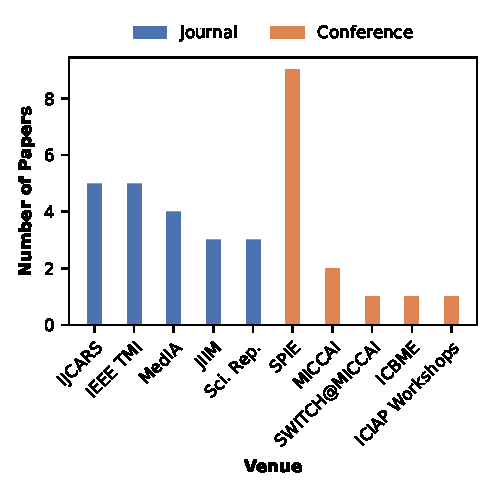
\includegraphics[width=1\linewidth]{figs/venue_analysis_stacked.pdf}
\caption{Top publication venues by paper count, stratified by venue type. IJCARS: International Journal of Computer Assisted Radiology and Surgery; IEEE TMI: IEEE Transactions on Medical Imaging; MedIA: Medical Image Analysis; JIIM: Journal of Imaging Informatics in Medicine; Sci.\ Rep.: Scientific Reports; SPIE: Proceedings of SPIE; MICCAI: International Conference on Medical Image Computing and Computer-Assisted Intervention; SWITCH@MICCAI: SWITCH workshop at MICCAI; ICBME: Iranian Conference on Biomedical Engineering; JACC: Journal of the American College of Cardiology.}
\label{fig:venue_stacked}
\end{figure}
\begin{figure}[]
\centering
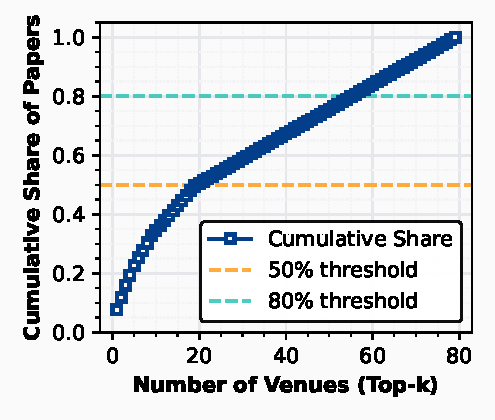
\includegraphics[width=1\linewidth]{figs/venue_cumulative_curve.pdf}
\caption{Cumulative share of studies across venues, ranked by study count. Dashed lines mark 50\% (yellow) and 80\% (green).}
\label{fig:venue_curve}
\end{figure}

Most studies are journal articles (89 of 120), with 24 conference papers and 7 preprints. The most frequent outlet is the SPIE proceedings (11 studies, 9 of them under the series name shown in Figure~\ref{fig:venue_stacked}), followed by IJCARS and IEEE TMI (5 each) and Medical Image Analysis (4). Among the 119 studies with a stated venue, half are spread across 20 venues, 56 of the 79 venues are needed to reach 80\%, and 60 venues contribute a single study (Figure~\ref{fig:venue_curve}). Engineering venues are well represented (11 studies in IEEE venues and 11 in SPIE proceedings), but MICCAI (three records) and ACM venues (none) are not, and conferences contribute far less here than in medical image computing generally.

\vspace{0.25cm}
\begin{mdframed}[linewidth=0.5pt, linecolor=black, backgroundcolor=blue!10]
\textbf{Finding 4.} No venue serves as a hub: the 120 studies are spread over 79 venues, 60 of which contribute a single study, so syntheses must search broadly.
\end{mdframed}
\vspace{0.25cm}

\subsection{Reported Performance}
\label{subsec:performance}
\begin{figure}[]
\centering
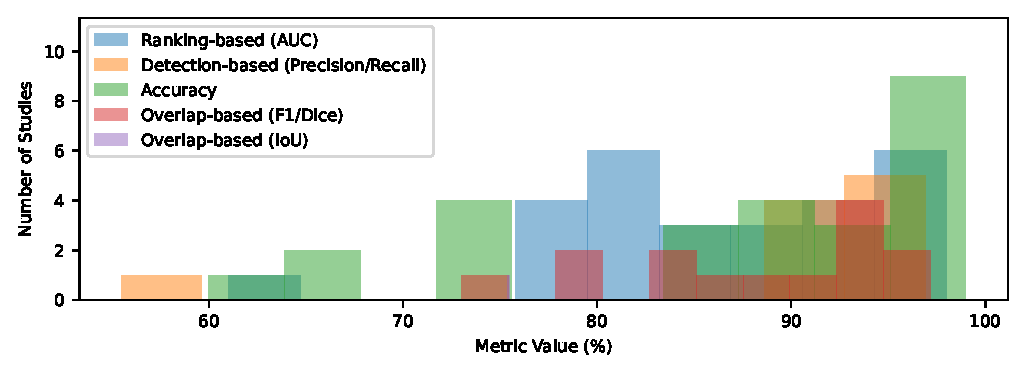
\includegraphics[width=1\linewidth]{figs/histogram_metrics.pdf}
\caption{Distribution of reported performance values by metric family.}
\label{fig:metric_histogram}
\end{figure}
\begin{figure}[]
\centering
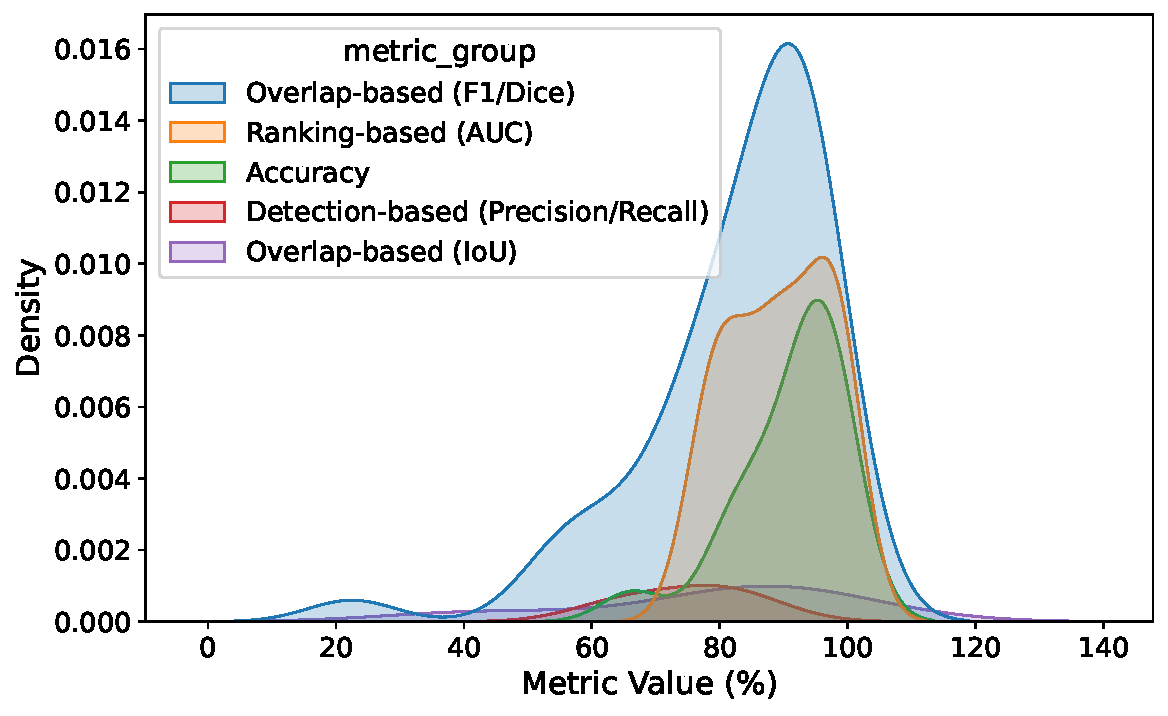
\includegraphics[width=1\linewidth]{figs/kde_metrics.pdf}
\caption{Kernel density estimates of reported performance values by metric family.}
\label{fig:metric_kde}
\end{figure}

Reported values are high in the four metric families used by more than one study, with family means between 86.6 and 89.9 on a 0--100 scale (Figures~\ref{fig:metric_histogram} and \ref{fig:metric_kde}). Accuracy (26 studies; SD 12.0, range 60--99) and detection precision and recall (10 studies; SD 12.5) are the most dispersed; Dice/F1 (14 studies; SD 7.5, range 73--97) and AUC (27 studies; SD 8.7) are tighter. Accuracy is also the least informative of these under the class imbalance common in angiographic tasks. With different datasets and protocols and no shared benchmark, these values cannot be compared across studies; the skew toward high values is consistent with publication bias and with testing on data similar to the training data.

\vspace{0.25cm}
\begin{mdframed}[linewidth=0.5pt, linecolor=black, backgroundcolor=blue!10]
\textbf{Finding 5.} Reported performance is consistently high but not comparable across studies, because datasets, protocols and metrics differ and no shared benchmark exists.
\end{mdframed}
\vspace{0.25cm}

\subsection{Reporting Quality and Clinical Readiness}
\label{subsec:reporting_quality}
\begin{figure*}[]
\centering
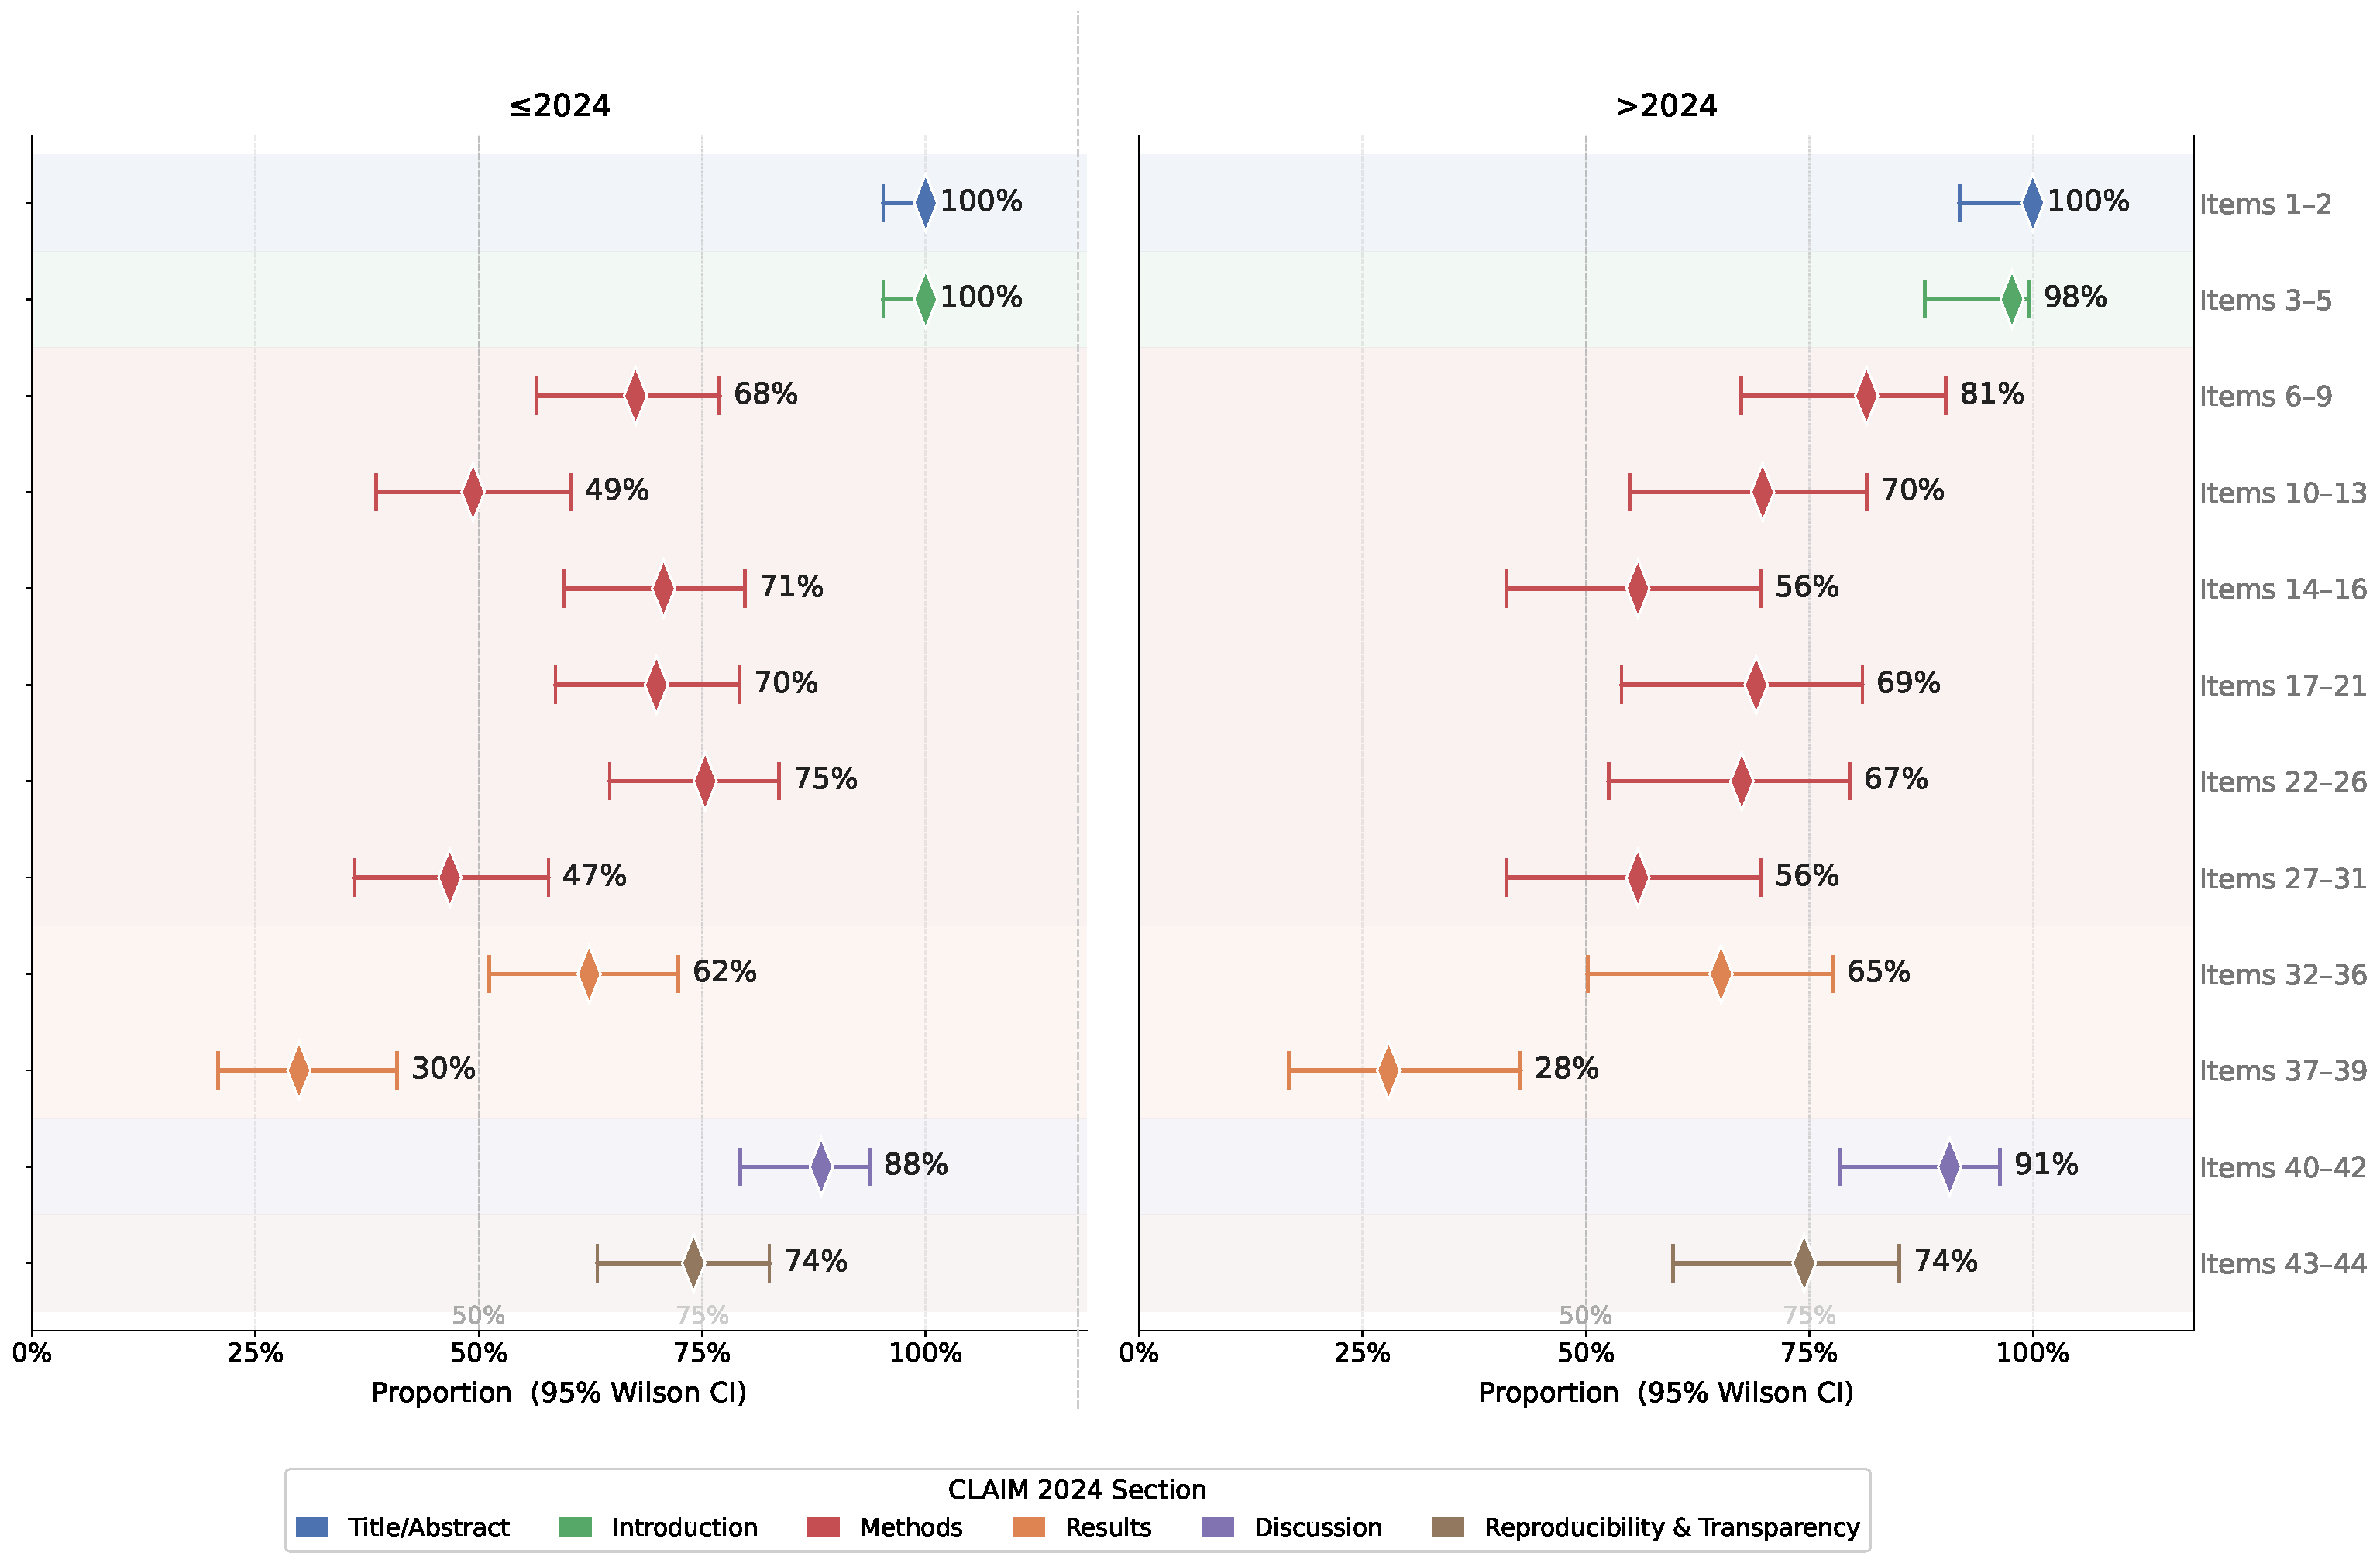
\includegraphics[width=1\linewidth]{figs/forest_plot_claim2024_comparison.pdf}
\caption{CLAIM 2024 adherence by cluster for studies published up to 2024 (left) and from 2025 onward (right). Diamonds show the proportion of studies meeting each cluster, with 95\% Wilson confidence intervals; colors mark the CLAIM section, and the right axis lists the checklist items in each cluster~\cite{Tejani2024}.}
\label{fig:forest_plot}
\end{figure*}

\definecolor{claimTA}{HTML}{4C72B0}
\definecolor{claimIntro}{HTML}{55A868}
\definecolor{claimMeth}{HTML}{C44E52}
\definecolor{claimRes}{HTML}{DD8452}
\definecolor{claimDisc}{HTML}{8172B2}
\definecolor{claimRepro}{HTML}{937860}

\begin{table}[ht]
  \centering
  \caption{CLAIM 2024 Adherence by Thematic Cluster: Temporal Comparison
    ($\leq 2024$ vs.\ $\geq 2025$).}
  \label{tab:claim2024_temporal}

  \footnotesize
  \renewcommand{\arraystretch}{1.25}
  \setlength{\tabcolsep}{4pt}

  \resizebox{\columnwidth}{!}{%
  \begin{tabular}{@{}
      l
      p{6.2cm}
      r r
      r r
      >{\centering\arraybackslash}p{1.2cm}
  @{}}

    \toprule

    \multicolumn{1}{l}{\textbf{ID}} &
    \multicolumn{1}{l}{\textbf{Cluster}} &
    \multicolumn{2}{c}{$\boldsymbol{\leq 2024}$ \textbf{(N\,=\,127)}} &
    \multicolumn{2}{c}{$\boldsymbol{\geq 2025}$ \textbf{(N\,=\,56)}} &
    \multicolumn{1}{c}{$\boldsymbol{\Delta}$} \\

    \cmidrule(lr){3-4}
    \cmidrule(lr){5-6}

    & &
    \textbf{\%} & \textbf{95\% CI} &
    \textbf{\%} & \textbf{95\% CI} &
    \\

    \midrule

    \rowcolor{claimTA!15}
    \multicolumn{7}{l}{\textbf{\textcolor{claimTA}{Title/Abstract}}} \\

    C01 & AI identification \& abstract completeness
    & 71\% & [62, 78]
    & 75\% & [62, 84]
    & $+4\%$~$\uparrow$ \\

    \midrule

    \rowcolor{claimIntro!15}
    \multicolumn{7}{l}{\textbf{\textcolor{claimIntro}{Introduction}}} \\

    C02 & Background \& study objectives
    & 98\% & [94, 100]
    & 98\% & [91, 100]
    & $\pm0\%$~$\sim$ \\

    \midrule

    \rowcolor{claimMeth!15}
    \multicolumn{7}{l}{\textbf{\textcolor{claimMeth}{Methods}}} \\

    C03 & Study design \& data sources
    & 42\% & [34, 50]
    & 61\% & [48, 72]
    & $+19\%$~$\uparrow$ \\

    C04 & Participants \& image acquisition
    & 29\% & [21, 37]
    & 38\% & [26, 51]
    & $+9\%$~$\uparrow$ \\

    C05 & Ground truth \& annotation
    & 31\% & [24, 40]
    & 46\% & [34, 59]
    & $+15\%$~$\uparrow$ \\

    C06 & Data partitioning \& class handling
    & 44\% & [36, 53]
    & 44\% & [31, 57]
    & $\pm0\%$~$\sim$ \\

    C07 & Model architecture \& training
    & 65\% & [56, 72]
    & 64\% & [50, 75]
    & $-1\%$~$\sim$ \\

    C08 & Evaluation design \& fairness
    & 24\% & [17, 32]
    & 52\% & [39, 64]
    & $+28\%$~$\uparrow$ \\

    \midrule

    \rowcolor{claimRes!15}
    \multicolumn{7}{l}{\textbf{\textcolor{claimRes}{Results}}} \\

    C09 & Performance \& external validation
    & 35\% & [27, 44]
    & 44\% & [31, 57]
    & $+9\%$~$\uparrow$ \\

    C10 & Demographic \& subgroup reporting
    & 8\% & [4, 14]
    & 16\% & [9, 28]
    & $+8\%$~$\uparrow$ \\

    \midrule

    \rowcolor{claimDisc!15}
    \multicolumn{7}{l}{\textbf{\textcolor{claimDisc}{Discussion}}} \\

    C11 & Limitations, implications \& future work
    & 84\% & [77, 90]
    & 89\% & [79, 95]
    & $+5\%$~$\uparrow$ \\

    \midrule

    \rowcolor{claimRepro!15}
    \multicolumn{7}{l}{\textbf{\textcolor{claimRepro}{Reproducibility \& Transparency}}} \\

    C12 & Reproducibility \& funding disclosure
    & 21\% & [15, 29]
    & 23\% & [14, 36]
    & $+2\%$~$\sim$ \\

    \bottomrule

    \multicolumn{7}{p{\hsize}}{%
      \textit{Note:} Proportions are the fraction of studies reporting adherence
      (``Yes'') among those where the item was applicable (NA excluded).
      95\% Wilson confidence intervals are shown.
      $\Delta$ = post--pre difference; arrows indicate changes greater than
      2 percentage points.
    } \\

  \end{tabular}%
  }

\end{table}
% \definecolor{claimTA}{HTML}{4C72B0}
% \definecolor{claimIntro}{HTML}{55A868}
% \definecolor{claimMeth}{HTML}{C44E52}
% \definecolor{claimRes}{HTML}{DD8452}
% \definecolor{claimDisc}{HTML}{8172B2}
% \definecolor{claimRepro}{HTML}{937860}

% \begin{table}[ht]
%   \centering
%   \caption{CLAIM 2024 Adherence by Thematic Cluster: Temporal Comparison
%     ($\leq 2024$ vs.\ $\geq 2025$).}
%   \label{tab:claim2024_temporal}

%   \footnotesize
%   \renewcommand{\arraystretch}{1.25}
%   \setlength{\tabcolsep}{4pt}

%   \resizebox{\columnwidth}{!}{%
%   \begin{tabular}{@{}
%       l
%       p{6.2cm}
%       r r
%       r r
%       >{\centering\arraybackslash}p{1.2cm}
%   @{}}

%     \toprule

%     \multicolumn{1}{l}{\textbf{ID}} &
%     \multicolumn{1}{l}{\textbf{Cluster}} &
%     \multicolumn{2}{c}{$\boldsymbol{\leq 2024}$ \textbf{(N\,=\,127)}} &
%     \multicolumn{2}{c}{$\boldsymbol{\geq 2025}$ \textbf{(N\,=\,56)}} &
%     \multicolumn{1}{c}{$\boldsymbol{\Delta}$} \\

%     \cmidrule(lr){3-4}
%     \cmidrule(lr){5-6}

%     & &
%     \textbf{\%} & \textbf{95\% CI} &
%     \textbf{\%} & \textbf{95\% CI} &
%     \\

%     \midrule

%     \rowcolor{claimTA!15}
%     \multicolumn{7}{l}{\textbf{\textcolor{claimTA}{Title/Abstract}}} \\

%     C01 & AI identification \& abstract completeness
%     & 71\% & [62, 78]
%     & 75\% & [62, 84]
%     & $+4\%$~$\uparrow$ \\

%     \midrule

%     \rowcolor{claimIntro!15}
%     \multicolumn{7}{l}{\textbf{\textcolor{claimIntro}{Introduction}}} \\

%     C02 & Background \& study objectives
%     & 98\% & [94, 100]
%     & 98\% & [91, 100]
%     & $\pm0\%$~$\sim$ \\

%     \midrule

%     \rowcolor{claimMeth!15}
%     \multicolumn{7}{l}{\textbf{\textcolor{claimMeth}{Methods}}} \\

%     C03 & Study design \& data sources
%     & 42\% & [34, 50]
%     & 61\% & [48, 72]
%     & $+19\%$~$\uparrow$ \\

%     C04 & Participants \& image acquisition
%     & 29\% & [21, 37]
%     & 38\% & [26, 51]
%     & $+9\%$~$\uparrow$ \\

%     C05 & Ground truth \& annotation
%     & 31\% & [24, 40]
%     & 46\% & [34, 59]
%     & $+15\%$~$\uparrow$ \\

%     C06 & Data partitioning \& class handling
%     & 44\% & [36, 53]
%     & 44\% & [31, 57]
%     & $\pm0\%$~$\sim$ \\

%     C07 & Model architecture \& training
%     & 65\% & [56, 72]
%     & 64\% & [50, 75]
%     & $-1\%$~$\sim$ \\

%     C08 & Evaluation design \& fairness
%     & 24\% & [17, 32]
%     & 52\% & [39, 64]
%     & $+28\%$~$\uparrow$ \\

%     \midrule

%     \rowcolor{claimRes!15}
%     \multicolumn{7}{l}{\textbf{\textcolor{claimRes}{Results}}} \\

%     C09 & Performance \& external validation
%     & 35\% & [27, 44]
%     & 44\% & [31, 57]
%     & $+9\%$~$\uparrow$ \\

%     C10 & Demographic \& subgroup reporting
%     & 8\% & [4, 14]
%     & 16\% & [9, 28]
%     & $+8\%$~$\uparrow$ \\

%     \midrule

%     \rowcolor{claimDisc!15}
%     \multicolumn{7}{l}{\textbf{\textcolor{claimDisc}{Discussion}}} \\

%     C11 & Limitations, implications \& future work
%     & 84\% & [77, 90]
%     & 89\% & [79, 95]
%     & $+5\%$~$\uparrow$ \\

%     \midrule

%     \rowcolor{claimRepro!15}
%     \multicolumn{7}{l}{\textbf{\textcolor{claimRepro}{Reproducibility \& Transparency}}} \\

%     C12 & Reproducibility \& funding disclosure
%     & 21\% & [15, 29]
%     & 23\% & [14, 36]
%     & $+2\%$~$\sim$ \\

%     \bottomrule

%     \multicolumn{7}{p{\hsize}}{%
%       \textit{Note:} Proportions are the fraction of studies reporting adherence
%       (``Yes'') among those where the item was applicable (NA excluded).
%       95\% Wilson confidence intervals are shown.
%       $\Delta$ = post--pre difference; arrows indicate changes greater than
%       2 percentage points.
%     } \\

%   \end{tabular}%
%   }

% \end{table}


We assessed all 120 studies against CLAIM 2024~\cite{Tejani2024}, the RSNA reporting checklist for AI in medical imaging (Figure~\ref{fig:forest_plot}, Table~\ref{tab:claim2024_temporal}). Background and objectives are reported almost universally; methods reporting is weaker and uneven. Between studies published up to 2024 and those from 2025 onward, the largest differences are in participant and image-acquisition reporting (C04: 49\% to 70\%, $p=0.04$), study design and data sources (C03: 68\% to 81\%, $p=0.14$) and ground-truth and annotation reporting, which declines (C05: 71\% to 56\%, $p=0.11$). Demographic and subgroup reporting stays low (C10: 30\% and 28\%). No difference remains significant after Holm correction (smallest adjusted $p=0.43$); with 43 recent studies, only large shifts would be detectable. Only 25 studies (20.8\%) share code and 3 (2.5\%) share data, although the reproducibility cluster (C12), which also counts funding disclosure, is met by 74\%. Evidence of clinical readiness is also thin: 19 studies (15.8\%) report external validation (one of them alongside a prospective deployment), 3 (2.5\%) a prospective design, 4 (3.3\%) clinical deployment or live use, and 4 (3.3\%) discuss regulatory requirements.

\vspace{0.25cm}
\begin{mdframed}[linewidth=0.5pt, linecolor=black, backgroundcolor=blue!10]
\textbf{Finding 6.} Reporting is strong for background and objectives but weak for subgroup analysis, code and data sharing, and has not changed measurably since CLAIM 2024.
\end{mdframed}
\vspace{0.25cm}

\subsection{Research Gaps and Future Research Implications}
\label{sec:research_gaps}

\begin{figure*}[htbp]
  \centering
  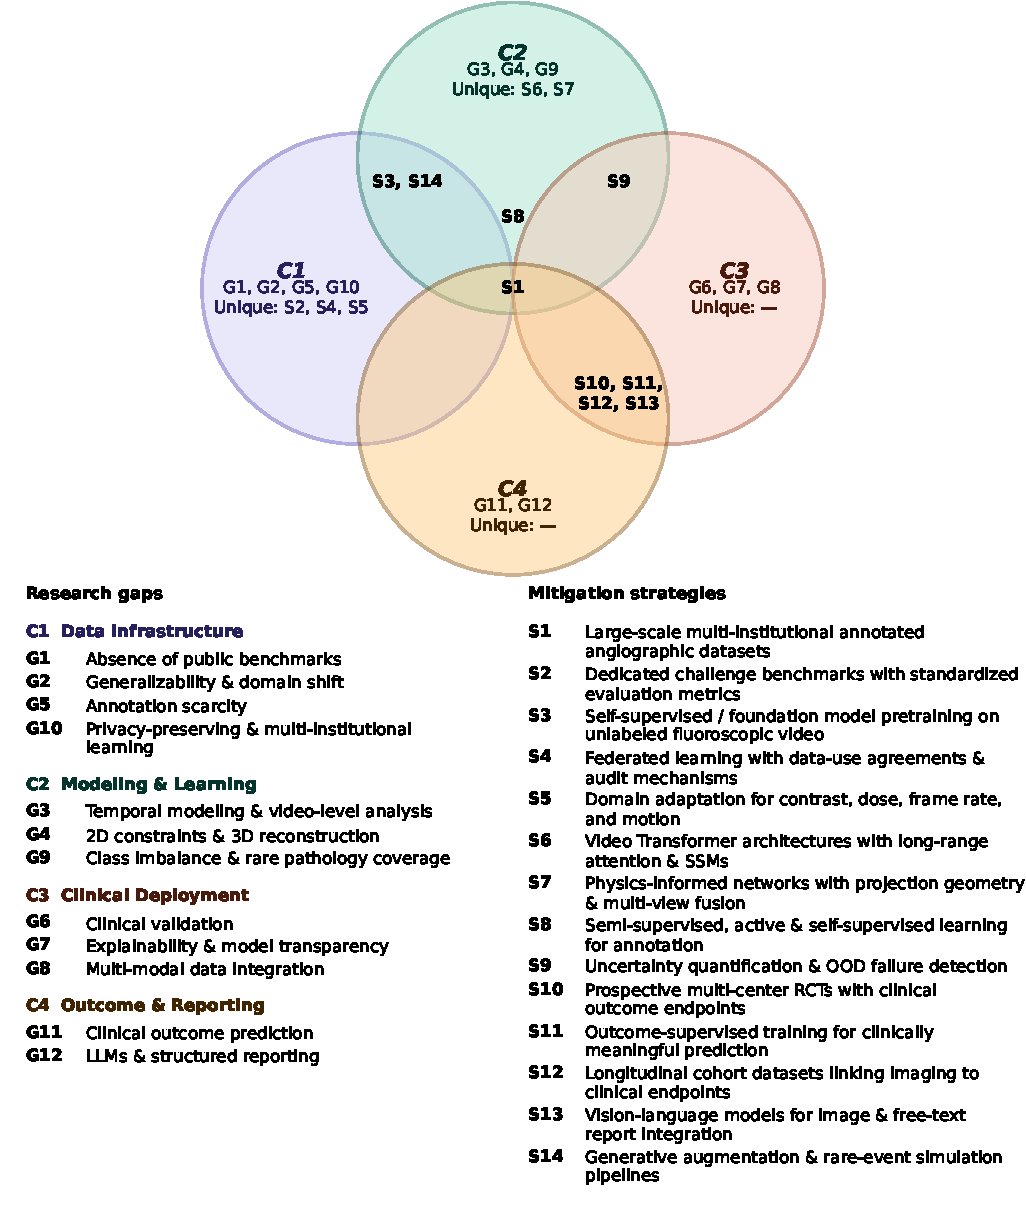
\includegraphics[height=11.5cm,width=\textwidth]{figs/venn_diagram.pdf}
  \caption{Thematic clustering of research gaps and mitigation strategies identified in the systematic review of AI-based angiographic and fluoroscopic image analysis. The four overlapping circles represent thematic clusters: \textbf{C1 --- Data Infrastructure} (gaps G1, G2, G10; lavender); \textbf{C2 --- Modeling \& Learning} (gaps G3, G4, G5, G9; green); \textbf{C3 --- Clinical Deployment} (gaps G6, G7, G8; salmon); and \textbf{C4 --- Outcome \& Reporting} (gaps G11, G12; amber). Overlap regions carry the strategy codes (S1--S14) shared across the intersecting clusters: the C1--C2 intersection is addressed by S1 (large-scale multi-institutional datasets); the C2--C3 intersection by S8 (annotation-efficient learning) and S9 (uncertainty quantification); and the C3--C4 intersection by S10--S13 (prospective
  trials, outcome-supervised training, longitudinal cohort datasets, and
  vision-language integration). Strategy S1 also is at the centre of
  all four clusters, reflecting its foundational role across every
  thematic domain. Strategies unique to each cluster are listed within
  the respective circle: C1 uniquely requires S2 (challenge benchmarks),
  S4 (federated learning), and S5 (domain adaptation); C2 uniquely
  requires S3 (foundation model pretraining), S6 (video Transformer
  architectures), S7 (physics-informed networks), and S14 (generative
  augmentation). Dashes (---) denote cluster intersections for which no
  shared strategy was identified across the reviewed literature. Gap and
  strategy codes correspond to the identifiers used throughout
  Table~\ref{tab:research_gaps} and the accompanying narrative.}
  \label{fig:venn_gaps}
\end{figure*}

Twelve research gaps identified across the 194 included studies can be organized into four thematic clusters that reflect the structural
layers at which the current literature exhibits shortcomings (Figure~\ref{fig:venn_gaps}). The first cluster, \textit{Data
Infrastructure} (C1), encompasses gaps in dataset size, public
availability, cross-institutional generalizability, and
privacy-preserving learning (G1, G2, G10); these are upstream constraints
whose resolution is a precondition for progress in every other area. The
second cluster, \textit{Modeling \& Learning} (C2), groups the
methodological gaps that limit what can be done even when data are
available: inadequate temporal modeling of angiographic video sequences,
the restriction to 2D projections, annotation scarcity, and class
imbalance (G3, G4, G5, G9). The third cluster, \textit{Clinical
Deployment} (C3), captures the gap between technical feasibility and
clinical readiness: the near-total absence of prospective validation, the
lack of model explainability, and the failure to integrate complementary
imaging modalities (G6, G7, G8). The fourth cluster, \textit{Outcome \&
Reporting} (C4), addresses the most distal translation gap: the
disconnection between imaging-level task performance and the clinical
outcome prediction and structured reporting capabilities that would make
AI tools genuinely useful at the point of care (G11, G12). As shown in
Figure~\ref{fig:venn_gaps}, these clusters are not independent. The
C1--C2 intersection is bridged by the construction of large-scale
annotated datasets (S1), which simultaneously enables better model
training and reduces annotation burden. The C2--C3 intersection is
addressed by annotation-efficient learning strategies (S8) and
uncertainty quantification frameworks (S9), both of which are
prerequisites for safe clinical deployment of models trained under data
constraints. The C3--C4 intersection is where prospective trial design
(S10), outcome-supervised training (S11), longitudinal cohort datasets
(S12), and vision-language integration (S13) converge, reflecting the
interdependence of clinical validation and outcome reporting. Strategy S1
occupies the centre of all four clusters because the availability of
large, diverse, well-annotated angiographic datasets is the single
intervention with the broadest leverage across every identified gap. Table~\ref{tab:research_gaps} details the evidence base for each gap and articulates
the corresponding future research directions.

% A systematic analysis of the limitations and future work directions
% reported across the 194 included studies reveals a set of recurring,
% structural deficiencies in the current state of artificial intelligence
% applied to angiographic and fluoroscopic imaging. Table~\ref{tab:research_gaps}
% consolidates the identified gaps and the corresponding proposed directions
% across twelve thematic research areas.

% ============================================================
% TABLE — portrait, no landscape required
% \small reduces font to ~8.5pt, giving ~15% more horizontal room.
% Column widths: 2.5 + 6.5 + 6.5 = 15.5 cm (fits A4 with 2 cm margins).
% \clearpage + \onecolumn escape two-column mode for longtable.
% \clearpage + \twocolumn restore it cleanly afterward.
% ============================================================
\clearpage
\onecolumn
\small

\begin{longtable}{>{\raggedright\arraybackslash}p{2.5cm}
                  >{\raggedright\arraybackslash}p{6.5cm}
                  >{\raggedright\arraybackslash}p{6.5cm}}

\caption{Evidence-driven research gaps and proposed future directions
identified from the systematic review of AI-based angiographic and
fluoroscopic image analysis.}
\label{tab:research_gaps} \\

\toprule
\textbf{Research Gaps} & \textbf{Evidence from the Literature} &
\textbf{Mitigation Strategies} \\
\midrule
\endfirsthead

\multicolumn{3}{c}{\tablename~\thetable{} --
  \textit{continued from previous page}} \\
\toprule
\textbf{Research Area} & \textbf{Identified Gap} &
\textbf{Mitigation Strategies} \\
\midrule
\endhead

\midrule
\multicolumn{3}{r}{\textit{Continued on next page}} \\
\endfoot

\bottomrule
\endlastfoot

% ---- Row 1 ----
\textbf{G1:} Absence of Public Benchmarks
&
\tabitem Small, private, single-center datasets dominate; most cohorts contain fewer than 200 patients \cite{ref20,ref24,ref41,ref45,ref71,ref72,ref78,ref79,ref85,ref86}.\newline
\tabitem No publicly available, annotated benchmark dataset specific to angiographic imaging exists \cite{ref4,ref15,ref27,ref34,ref50,ref56,ref63}.\newline
\tabitem Absence of shared benchmarks makes cross-study comparison practically impossible \cite{ref6,ref11,ref26,ref33,ref38,ref49,ref57,ref58,ref87,ref97,ref98,ref99}.\newline
\tabitem Inconsistent evaluation protocols prevent measurement of field-wide progress \cite{ref1,ref65,ref89}.
&
\tabitem Construct and release large-scale multi-institutional angiographic datasets with standardized pixel-level annotations and defined train/test splits \cite{ref15,ref29,ref63,ref75,ref94}.\newline
\tabitem Organize dedicated challenge benchmarks modeled on established medical image segmentation competitions \cite{ref2,ref39}.\newline
\tabitem Mandate inter-rater reliability protocols in annotation guidelines to ensure label quality \cite{ref19}.\newline
\tabitem Define standard evaluation metrics and phantom-versus-patient evaluation subsets \cite{ref29}.
\\
\dashedrule

% ---- Row 2 ----
\textbf{G2:} Generalizability \& Domain Shift
&
\tabitem Models trained on a single vendor or acquisition protocol consistently fail to transfer to external settings \cite{ref5,ref9,ref10,ref15,ref27,ref29,ref38,ref83,ref93}.\newline
\tabitem Domain shift between synthetic training data and real clinical images remains unresolved \cite{ref52,ref64,ref74}.\newline
\tabitem Methods validated on coronary angiography degrade when applied to cerebral, renal, or peripheral vasculature \cite{ref16,ref40,ref56,ref62,ref63,ref65,ref75,ref81}.\newline
\tabitem Multi-center heterogeneity in frame rate, contrast dosing, and radiation settings is rarely addressed \cite{ref14,ref17,ref19,ref23,ref25,ref51,ref92,ref95}.
&
\tabitem Treat external multi-institutional validation as a required component, not an optional addition \cite{ref15,ref19,ref75}.\newline
\tabitem Develop domain adaptation methods tailored to variable contrast concentration, dose, frame rate, and motion profiles \cite{ref17,ref64}.\newline
\tabitem Extend personalized federated learning frameworks to accommodate non-identical cross-center data distributions \cite{ref19}.\newline
\tabitem Establish domain shift benchmarks to quantify performance degradation across imaging vendors \cite{ref5,ref64}.
\\
\dashedrule

% ---- Row 3 ----
\textbf{G3:} Temporal Modeling \& Video-Level Analysis
&
\tabitem Most methods treat each frame as an independent 2D image, discarding hemodynamic flow and contrast propagation dynamics \cite{ref31,ref50,ref52,ref58,ref65,ref93}.\newline
\tabitem Temporal models are typically restricted to short fixed-length clips, not full variable-length sequences \cite{ref10,ref34,ref36,ref67}.\newline
\tabitem Procedural phase transitions during interventional procedures are not explicitly modeled \cite{ref25,ref48,ref65}.\newline
\tabitem Respiratory and cardiac motion are treated as noise rather than informative temporal signals \cite{ref18,ref77,ref96}.
&
\tabitem Develop architectures that model the complete temporal structure of angiographic acquisitions, including mask, injection, and washout phases \cite{ref32,ref34,ref66}.\newline
\tabitem Evaluate video Transformer architectures with long-range attention and state-space models for efficient long-sequence processing \cite{ref25,ref66,ref93}.\newline
\tabitem Explore temporal self-supervised pretraining on large archives of unannotated fluoroscopic video \cite{ref18}.\newline
\tabitem Incorporate explicit hemodynamic priors into temporal model design \cite{ref77}.
\\
\dashedrule

% ---- Row 4 ----
\textbf{G4:} 2D Constraints \& 3D Reconstruction
&
\tabitem Angiographic projections collapse 3D vascular anatomy, introducing foreshortening, vessel overlap, and depth loss \cite{ref1,ref31,ref35,ref40,ref66}.\newline
\tabitem The vast majority of methods operate exclusively on single-plane 2D projections \cite{ref23,ref33,ref44,ref62}.\newline
\tabitem Robust 3D reconstruction from monoplane or biplane projections under intraoperative time constraints remains unsolved \cite{ref43,ref54,ref55,ref90}.\newline
\tabitem 2D/3D registration accuracy is insufficient for routine intraoperative use \cite{ref55,ref82}.
&
\tabitem Develop multi-view learning architectures that fuse information across projection angles \cite{ref23,ref66,ref90}.\newline
\tabitem Investigate physics-informed networks incorporating known projection geometry and contrast agent kinetics \cite{ref43,ref55}.\newline
\tabitem Leverage rotational angiographic acquisitions for temporally informed 3D reconstruction \cite{ref54,ref82}.\newline
\tabitem Systematically combine intraoperative cone-beam CT with fluoroscopic AI pipelines to provide 3D context \cite{ref21}.
\\
\dashedrule

% ---- Row 5 ----
\textbf{G5:} Annotation Scarcity \& Annotation-Efficient Learning
&
\tabitem Manual annotation requires substantial physician time and specialized expertise per labeled study \cite{ref2,ref13,ref34,ref67,ref87,ref97,ref98,ref99}.\newline
\tabitem Annotation is subject to significant intra- and inter-observer variability, rarely quantified in included studies \cite{ref4,ref11,ref46,ref56,ref58}.\newline
\tabitem Synthetic data generation partially addresses scarcity, but synthetic-to-real domain gaps persist \cite{ref52,ref64,ref74,ref98}.\newline
\tabitem Semi-supervised and self-supervised methods are underrepresented across angiographic analysis tasks \cite{ref18,ref49}.
&
\tabitem Systematically evaluate semi-supervised, self-supervised, and active learning strategies with explicit performance-versus-label-count analysis \cite{ref2,ref49,ref74}.\newline
\tabitem Pursue foundation model pretraining on large archives of unlabeled fluoroscopic video \cite{ref18}.\newline
\tabitem Validate generative data augmentation methods informed by realistic vascular anatomy models and imaging physics \cite{ref52,ref64}.\newline
\tabitem Develop annotation tools that integrate uncertainty estimation to prioritize the most informative cases for expert labeling \cite{ref46}.
\\
\dashedrule

% ---- Row 6 ----
\textbf{G6:} Prospective Clinical Validation \& Outcome Assessment
&
\tabitem Nearly all included studies rely on retrospective analysis of previously acquired images \cite{ref14,ref26,ref42,ref53,ref59,ref61,ref76,ref84,ref91}.\newline
\tabitem Prospective validation in live clinical settings is almost entirely absent from the literature \cite{ref1,ref7,ref16,ref25,ref49,ref51,ref65}.\newline
\tabitem Retrospective evaluation cannot measure the effect of AI outputs on physician behavior or patient outcomes \cite{ref37,ref68,ref70}.\newline
\tabitem Demonstrated technical performance does not establish clinical value or cost-effectiveness \cite{ref53,ref65}.
&
\tabitem Design prospective clinical evaluation frameworks in collaboration between AI researchers and clinicians from the outset \cite{ref14,ref42}.\newline
\tabitem Pursue randomized controlled trials comparing outcomes under standard-of-care versus AI-assisted decision-making \cite{ref25,ref76}.\newline
\tabitem Engage regulatory bodies early to define the evidence standards required for clinical deployment \cite{ref39,ref59}.\newline
\tabitem Develop AI interface designs that integrate model outputs into existing workflow without adding cognitive burden \cite{ref84}.
\\
\dashedrule

% ---- Row 7 ----
\textbf{G7:} Explainability \& Model Transparency
&
\tabitem Most deep learning models produce predictions without clinically interpretable justification \cite{ref14,ref65}.\newline
\tabitem Existing attention visualization approaches provide limited mechanistic insight \cite{ref68,ref89}.\newline
\tabitem Silent failure modes in out-of-distribution inputs are a particular concern for patient safety \cite{ref25}.\newline
\tabitem Regulatory and clinical trust requirements are not satisfied by aggregate performance metrics alone \cite{ref14,ref89}.
&
\tabitem Treat uncertainty quantification as a core design requirement, communicating confidence alongside every prediction \cite{ref14,ref25}.\newline
\tabitem Develop failure detection systems that flag out-of-distribution inputs for mandatory human review \cite{ref25,ref68}.\newline
\tabitem Design intermediate representations aligned with clinically meaningful anatomical and hemodynamic concepts \cite{ref68}.\newline
\tabitem Evaluate whether explainability outputs demonstrably improve clinical decision-making in prospective user studies \cite{ref89}.
\\
\dashedrule

% ---- Row 8 ----
\textbf{G8:} Multi-Modal Data Integration
&
\tabitem Studies predominantly process angiographic images in isolation, discarding complementary clinical data \cite{ref16,ref32,ref62}.\newline
\tabitem Pressure wire measurements, IVUS, OCT, CTA, ECG, and laboratory biomarkers are routinely available but unused \cite{ref30,ref46,ref69,ref81,ref91}.\newline
\tabitem Missing modalities at inference time, common in clinical practice, are rarely addressed \cite{ref25,ref84}.\newline
\tabitem Longitudinal multi-modal datasets linking intraoperative imaging to procedural outcomes are essentially absent \cite{ref21}.
&
\tabitem Develop architectures capable of fusing imaging, hemodynamic, and structured clinical data with explicit handling of missing modalities \cite{ref25,ref32}.\newline
\tabitem Construct longitudinal multi-modal cohort datasets linking angiographic sequences to post-procedural outcomes \cite{ref21,ref91}.\newline
\tabitem Explore vision-language model architectures for integrating free-text clinical notes with imaging features \cite{ref30}.\newline
\tabitem Define outcome-oriented multi-modal training objectives that directly optimize for clinically meaningful predictions \cite{ref46,ref69}.
\\
\dashedrule

% ---- Row 9 ----
\textbf{G9:} Class Imbalance \& Rare Pathology Coverage
&
\tabitem Rare events such as vessel perforation, intracranial aneurysm, and gastrointestinal bleeding are severely underrepresented \cite{ref20,ref21,ref80}.\newline
\tabitem Standard training objectives produce models biased toward majority classes with poor sensitivity for critical minority cases \cite{ref4,ref25,ref57,ref65,ref79,ref89}.\newline
\tabitem Rare anatomical variants and complex lesion morphologies are systematically excluded from study cohorts \cite{ref47,ref50,ref87}.\newline
\tabitem Aggregate performance metrics obscure minority-class failure, masking clinically important shortcomings \cite{ref80,ref89}.
&
\tabitem Systematically evaluate oversampling, cost-sensitive learning, hard negative mining, and generative augmentation across imbalance ratios \cite{ref4,ref80}.\newline
\tabitem Explicitly target underrepresented pathology types in dataset construction rather than excluding them \cite{ref20}.\newline
\tabitem Mandate stratified reporting of performance metrics for rare classes alongside aggregate figures \cite{ref80}.\newline
\tabitem Develop rare-event simulation pipelines for synthetic augmentation of clinically critical minority cases \cite{ref80}.
\\
\dashedrule

% ---- Row 10 ----
\textbf{G10:} Privacy-Preserving \& Multi-Institutional Learning
&
\tabitem Patient privacy regulations and data governance barriers prevent centralization of large angiographic datasets \cite{ref14,ref15,ref75}.\newline
\tabitem Federated learning for angiographic analysis is barely represented in the reviewed literature; only one study explicitly adopts this framework \cite{ref19}.\newline
\tabitem Non-identical data distributions across institutions complicate federated model training \cite{ref19,ref92}.\newline
\tabitem Auditability and accountability requirements for federated clinical AI systems are unaddressed \cite{ref14}.
&
\tabitem Develop federated learning frameworks specifically tailored to large angiographic video inputs with efficient communication protocols \cite{ref19}.\newline
\tabitem Evaluate differential privacy and secure multi-party computation approaches for their impact on model utility \cite{ref19}.\newline
\tabitem Establish standardized data use agreements and federated audit mechanisms for cross-institutional AI training \cite{ref15,ref19}.\newline
\tabitem Benchmark personalized federated approaches against centralized baselines as a function of institutional data heterogeneity \cite{ref19}.
\\
\dashedrule

% ---- Row 11 ----
\textbf{G11}: Imaging Biomarkers \& Clinical Outcome Prediction
&
\tabitem Most methods focus on intermediate imaging tasks rather than on direct clinical outcome prediction \cite{ref1,ref14,ref25,ref69,ref84}.\newline
\tabitem Demonstrating detection or segmentation accuracy does not establish impact on revascularization decisions or survival \cite{ref42,ref59,ref91}.\newline
\tabitem Longitudinal cohort designs linking imaging findings to follow-up clinical endpoints are largely absent \cite{ref71,ref72,ref76}.\newline
\tabitem Outcome-supervised training objectives have not been systematically explored in the angiographic domain \cite{ref84,ref91}.
&
\tabitem Construct longitudinal datasets linking intraoperative angiographic images to post-procedural endpoints including re-intervention rates and mortality \cite{ref42,ref76}.\newline
\tabitem Develop outcome-supervised training objectives that directly optimize for clinically meaningful event prediction \cite{ref14,ref84}.\newline
\tabitem Apply imaging biomarker discovery workflows combining feature extraction with survival and outcome modeling \cite{ref59,ref71,ref72}.\newline
\tabitem Integrate procedural databases and electronic health record data with angiographic image archives to enable outcome-linked training \cite{ref84,ref91}.
\\
\dashedrule

% ---- Row 12 ----
\textbf{G12}: Large Language Models \& Structured Reporting
&
\tabitem LLM application to angiographic reporting and clinical knowledge integration is almost entirely unexplored; only one study in this review addresses this area \cite{ref73}.\newline
\tabitem Free-text angiographic reports contain rich structured information routinely discarded in downstream analyses \cite{ref73}.\newline
\tabitem The only included study on LLM-based report structuring is geographically restricted to Korean institutions and relies on proprietary models, limiting reproducibility \cite{ref73}.\newline
\tabitem Multimodal vision-language models for integrated image-and-report reasoning have not been evaluated in this domain \cite{ref73}.
&
\tabitem Evaluate open-source LLMs and vision-language models for angiographic report structuring, finding extraction, and downstream decision support \cite{ref73}.\newline
\tabitem Develop end-to-end pipelines that integrate structured imaging outputs with natural language generation for automated report synthesis \cite{ref73}.\newline
\tabitem Construct standardized angiographic reporting ontologies to provide a shared vocabulary for cross-institutional NLP model training \cite{ref73}.\newline
\tabitem Benchmark open-source models against proprietary baselines on diverse international angiographic report corpora \cite{ref73}.
\\

\end{longtable}

\subsection{Toward an Actionable Roadmap}
\label{sec:actionable_roadmap}

While Table~\ref{tab:research_gaps} documents the evidence base and candidate mitigation strategies for each gap, it does not by itself prioritize where the field should act first or specify how progress could be measured. Table~\ref{tab:cbm_roadmap} distills this analysis into a compact, actionable roadmap: for each gap, it reports the number of included studies documenting the gap in the literature (Evidence Count, computed directly from the citations underlying Table~\ref{tab:research_gaps}), the clinical risk of leaving the gap unaddressed, the corresponding computational opportunity, and a concrete benchmark or evaluation recommendation that would make progress on the gap measurable. Gaps with the largest evidence bases (G1, G2, G6) represent the most extensively documented structural barriers in the current literature, whereas gaps with a narrow evidence base (G7, G10, G12) reflect emerging but still underexplored directions.

\footnotesize
\begin{longtable}{>{\raggedright\arraybackslash}p{2.1cm}
                  >{\centering\arraybackslash}p{1.1cm}
                  >{\raggedright\arraybackslash}p{4.1cm}
                  >{\raggedright\arraybackslash}p{4.1cm}
                  >{\raggedright\arraybackslash}p{4.3cm}}

\caption{CBM-facing actionable roadmap synthesizing each research gap identified in Table~\ref{tab:research_gaps} into clinical risk, computational opportunity, and a concrete benchmark or evaluation recommendation. Evidence Count is the number of distinct included studies cited as documenting each gap in Table~\ref{tab:research_gaps}.}
\label{tab:cbm_roadmap} \\

\toprule
\textbf{Gap} & \textbf{Evid.\ Count} & \textbf{Clinical Risk} & \textbf{Computational Opportunity} & \textbf{Benchmark / Evaluation Recommendation} \\
\midrule
\endfirsthead

\multicolumn{5}{c}{\tablename~\thetable{} -- \textit{continued from previous page}} \\
\toprule
\textbf{Gap} & \textbf{Evid.\ Count} & \textbf{Clinical Risk} & \textbf{Computational Opportunity} & \textbf{Benchmark / Evaluation Recommendation} \\
\midrule
\endhead

\midrule
\multicolumn{5}{r}{\textit{Continued on next page}} \\
\endfoot

\bottomrule
\endlastfoot

\textbf{G1} Absence of Public Benchmarks & 32 &
Reported performance cannot be verified to generalize beyond the originating institution before deployment, risking undetected failure in new clinical settings. &
Large-scale, standardized, publicly released multi-institutional datasets with defined train/test splits. &
Organize a public challenge benchmark with standardized metrics and phantom-versus-patient evaluation subsets. \\
\dashedrule

\textbf{G2} Generalizability \& Domain Shift & 28 &
Models validated at a single site, vendor, or vascular territory may silently degrade elsewhere, producing unreliable outputs during patient care without warning. &
Domain adaptation and personalized federated learning tailored to cross-vendor, cross-protocol, and cross-territory variation. &
Require external multi-institutional validation and report a domain-shift benchmark quantifying degradation across imaging vendors. \\
\dashedrule

\textbf{G3} Temporal Modeling \& Video-Level Analysis & 15 &
Discarding hemodynamic flow and contrast-propagation dynamics risks missing clinically important temporal signals a frame-independent model cannot detect. &
Video-transformer and state-space architectures modeling full acquisition phases (mask, injection, washout) with hemodynamic priors. &
Evaluate on full variable-length real acquisitions with metrics scoring temporal fidelity, not accuracy on short fixed-length clips alone. \\
\dashedrule

\textbf{G4} 2D Constraints \& 3D Reconstruction & 14 &
Foreshortening, vessel overlap, and depth loss from monoplane 2D projections can cause missed or mis-measured lesions during intraoperative decisions. &
Multi-view and physics-informed 3D reconstruction from mono-/biplane or rotational angiographic acquisitions. &
Standardized 2D/3D registration accuracy benchmark evaluated under intraoperative time constraints. \\
\dashedrule

\textbf{G5} Annotation Scarcity \& Annotation-Efficient Learning & 18 &
Reliance on scarce expert annotation with unquantified inter-observer variability threatens label reliability for safety-critical model training. &
Semi-/self-supervised and active learning, foundation-model pretraining on large archives of unlabeled fluoroscopic video. &
Report performance-versus-label-count curves for each annotation-efficient method, rather than accuracy at a single fixed label budget. \\
\dashedrule

\textbf{G6} Prospective Clinical Validation \& Outcome Assessment & 19 &
Because almost no studies validate prospectively, there is no evidence these models change physician behavior or patient outcomes in live care. &
Prospective evaluation frameworks and outcome-supervised training designed jointly with clinicians from the outset. &
Randomized controlled trials comparing standard-of-care versus AI-assisted decision-making as the evaluation standard. \\
\dashedrule

\textbf{G7} Explainability \& Model Transparency & 5 &
Predictions without interpretable justification, and unflagged out-of-distribution failures, can silently mislead clinicians and undermine patient safety. &
Uncertainty quantification and failure-detection systems flagging out-of-distribution inputs for mandatory human review. &
Prospective user studies testing whether explainability outputs measurably improve clinical decision-making, not qualitative attention maps alone. \\
\dashedrule

\textbf{G8} Multi-Modal Data Integration & 11 &
Ignoring routinely available complementary data (IVUS, OCT, ECG, labs) means models may miss clinically decisive information a clinician would normally use. &
Fusion architectures with explicit handling of missing modalities; vision-language integration of free-text clinical notes. &
Outcome-oriented multi-modal benchmarks that explicitly test performance under missing-modality conditions. \\
\dashedrule

\textbf{G9} Class Imbalance \& Rare Pathology Coverage & 12 &
Models biased toward majority classes may have poor sensitivity for rare but critical events (e.g., perforation, aneurysm) -- precisely the cases where failure is most dangerous. &
Cost-sensitive learning, hard negative mining, and rare-event simulation or generative augmentation. &
Mandate stratified per-class sensitivity reporting for rare pathologies alongside aggregate accuracy metrics. \\
\dashedrule

\textbf{G10} Privacy-Preserving \& Multi-Institutional Learning & 5 &
Data governance barriers blocking multi-institutional pooling constrain how representative and safe models can be before wide deployment. &
Federated learning frameworks and differential privacy / secure multi-party computation for angiographic video. &
Benchmark personalized federated approaches against centralized baselines as a function of institutional data heterogeneity. \\
\dashedrule

\textbf{G11} Imaging Biomarkers \& Clinical Outcome Prediction & 11 &
Strong segmentation or detection accuracy does not establish that a model improves revascularization decisions or survival, so technical success may not translate to patient benefit. &
Outcome-supervised training objectives and imaging-biomarker discovery combined with survival modeling. &
Longitudinal cohort evaluation linking imaging-derived predictions to real clinical endpoints (re-intervention rate, mortality), not intermediate task metrics alone. \\
\dashedrule

\textbf{G12} Large Language Models \& Structured Reporting & 1 &
With only one included study (geographically and model-restricted), there is essentially no evidence base for LLM-assisted angiographic reporting, so its safety and reliability for clinical use is unknown. &
Open-source LLM and vision-language pipelines for angiographic report structuring and finding extraction. &
Benchmark open-source against proprietary models on diverse international angiographic report corpora using a standardized reporting ontology. \\

\end{longtable}
\normalsize

\clearpage
\twocolumn




\section{Discussion}\label{sec:discussion}

\subsection{Principal Findings}

This systematic literature review examined 120 studies of computational methods for angiographic sequence analysis. In this review, we found that publications increased rapidly after 2020, with 78\% appearing from 2022 onward. However, shared evaluation, reproducibility, and clinical validation remain limited in the reviewed corpus. The main findings of this manuscript have been summarized in four key takeaways:

First, temporal information is commonly used, but the way it is modeled varies substantially. Because eligibility required temporally ordered multi-frame data, these proportions characterize the selected sequence-analysis literature rather than angiographic AI as a whole. Although 97 studies (80.8\%) used sequential data, 49 use fixed operations and only 48 learn temporal representations. Learned temporal models are concentrated in classification tasks and remain scarce in flow analysis, device tracking, and outcome prediction. Moreover, 41 studies use short frame stacks rather than complete acquisitions, and 51 of the 97 studies that used sequential data still identify limited temporal modeling as a limitation. As shown in Table~\ref{tab:temporal_taxonomy}, using sequence data therefore covers approaches with very different temporal capabilities. The next research step is therefore to evaluate when learned temporal representations improve on simpler methods through controlled comparisons using the same data, inputs, and evaluation protocol.

Second, the literature is concentrated in a small number of clinical settings. Cardiac and neurologic applications constitute nearly 90\% of the included studies, and only five studies use both DSA and fluoroscopy. Evidence from these settings does not establish performance in other vascular territories or acquisition conditions. Broader evaluation should therefore include differences in anatomy, imaging vendors, frame rates, and acquisition protocols, rather than relying only on additional data from the development setting.

Third, reported performance is generally high, but its interpretation is limited by inconsistent evaluation. Public datasets are used by 20 studies, yet only three release their own data, and there is no common evaluation framework across the reviewed tasks. Differences in datasets, reference standards, and metrics make cross-study rankings unreliable. Therefore, public data benchmarks need to be built with defined test sets and consistent outcome definitions.

Fourth, evidence supporting clinical use remains limited. Only 19 studies report external validation, three use a prospective design, and four report clinical deployment or live use. These findings indicate that most evidence concerns technical performance rather than benefit during clinical care. Similarly, the reporting comparison shown in Figure~\ref{fig:forest_plot} found no statistically significant differences between studies published up to 2024 and those published from 2025 onward after Holm correction. This does not establish unchanged reporting or measure the effect of the CLAIM 2024 update.

The twelve research gaps bring these findings together. Table~\ref{tab:research_gaps} shows that model development is closely connected to data availability, annotation quality, evaluation, and clinical integration. Generalization, public benchmarks, and temporal modeling are the most frequently documented gaps, appearing in 68, 65, and 63 studies, respectively. These provide immediate priorities for further work. Federated learning, language models, and structured reporting are less represented and should be treated as directions requiring evaluation rather than established solutions.

\subsection{Comparison with Prior Work}

The surveys by Litjens et al.~\cite{Litjens2017} and Shen et al.~\cite{Shen2017} examine deep learning across medical imaging, while Moccia et al.~\cite{Moccia2018} review blood vessel segmentation, datasets, and evaluation metrics. Our review complements these perspectives by focusing on temporally ordered X-ray angiographic data and distinguishing fixed temporal operations from learned temporal representations. Using multiple frames may involve aggregation, registration, flow-curve fitting, or learning dependencies across a sequence; these approaches provide different temporal capabilities. Their frequency in the reviewed literature does not establish their effectiveness. Whether learned temporal models improve performance or clinical usefulness requires controlled comparisons using the same data, inputs, and evaluation protocol.

The reviews by Iezzi et al.~\cite{Iezzi2019}, Gurgitano et al.~\cite{Gurgitano2021}, and Mukhtar et al.~\cite{Mukhtar2025} examine AI across interventional radiology, including planning, guidance, interpretation, and clinical workflow. Our contribution is to examine data availability, external validation, evaluation, and clinical implementation within a defined corpus of angiographic sequence studies and relate them to tasks, architectures, and temporal modeling. We also assess reporting using review-specific criteria informed by CLAIM 2024~\cite{Tejani2024} (Appendix~\ref{app:claim_clusters}). Background and objectives were more consistently reported than demographics and subgroup performance; separately, code and data release were uncommon. Meeting the broader reproducibility and funding-disclosure cluster (C12) does not necessarily indicate artifact release. These findings distinguish reporting completeness and reproducibility resources from methodological validity and evidence of clinical usefulness.

\subsection{Limitations}
\label{sec:limitations}

First, the search covered only PubMed/\allowbreak MEDLINE and Semantic Scholar, up to 25 May 2026. PubMed searches were restricted to English, and each Semantic Scholar query was limited to its first 100 results. Conference papers and arXiv-only preprints may therefore be underrepresented. Publication counts for 2026 also cover only part of the year and should not be compared directly with full-year counts.

Second, title and abstract screening relied on an LLM. Two independent reviewers checked all 134 pipeline inclusions and a random sample of 357 exclusions, but most excluded records were not reviewed manually. Two eligible studies were found in the exclusion sample, giving an estimated 28 eligible records among the 4,930 original pipeline exclusions (95\% Wilson interval scaled to that stratum: 8--100), including the two records recovered by human review. Both failed the sequence-data criterion because their abstracts did not explicitly establish eligibility. The exclusion-by-default rules for I2 and I4 may therefore have reduced recall. The corpus is a validated sample of the retrieved literature rather than a complete census, and missed studies could affect category proportions as well as counts.

Third, full-text extraction relied on an LLM, and one reviewer audited six studies, representing 5\% of the corpus. Although 97.1\% of audited values were correct, this sample cannot establish the same accuracy for every field. Errors in interpretive categories, including temporal modeling and research gaps, may affect the synthesis. The gap analysis also depends on limitations and future directions stated by authors, so problems that were not explicitly discussed may be underrepresented.

Fourth, the reporting assessment used an operational schema informed by CLAIM 2024. As documented in Appendix~\ref{app:claim_clusters}, its 44 criteria do not consistently correspond to the numbering and definitions of the official checklist. The 12 thematic groups were defined for this review, and a group was counted as met when at least half of its applicable items were reported. These results should therefore be interpreted as reporting completeness under our schema, rather than strict adherence to the official CLAIM checklist. Group-level summaries may also conceal missing individual items. With 43 studies in the later publication period, the absence of statistically significant differences does not establish that reporting remained unchanged or that the guideline had no impact.

Fifth, we did not apply a dedicated risk-of-bias tool or conduct a meta-analysis. The reported performance distributions describe the extracted results but do not provide pooled estimates of generalization or clinical effectiveness. Differences in study settings and evaluation methods also prevent conclusions about whether one architecture or temporal modeling strategy is superior.

Finally, the review was not registered and had no published protocol. Full text was unavailable for two eligible studies, and three included records are earlier versions of another included study (R2434/R1238, R4154/R3555, and R4671/R4479 in \texttt{extraction/manifest.csv}). These related records introduce dependence and slightly inflate some counts.

\subsection{Conclusion}

This review shows growing interest in angiographic sequence analysis, with applications spanning classification, detection, segmentation, tracking, and image enhancement. Temporal information is widely used, but learned temporal representations remain concentrated in a few tasks. High reported performance is accompanied by limited data sharing, inconsistent evaluation, and little prospective evidence of clinical benefit.

Further progress requires shared multi-institutional datasets, task-specific benchmarks, controlled evaluation of temporal methods, and validation across vascular territories and acquisition settings. Prospective studies should then establish whether these methods improve clinical decisions, procedural workflow, or patient outcomes. These steps are necessary to turn technical improvements into reliable tools for angiography-guided care.

\section{Appendix A. Reproducible Search Log and Database-Specific Queries}
\label{appendix:search_log}

This appendix provides the exact, database-specific queries, execution dates, filters, and retrieval statistics used for the structured search described in Section~\ref{sec:eligibility}, to allow the search to be independently audited, reproduced, or extended to additional databases.

\subsection{PubMed/MEDLINE}

\textbf{Execution date:} 2026-05-25. \textbf{Interface:} NCBI Entrez E-utilities (\texttt{esearch}), via the Biopython \texttt{Bio.Entrez} client.

\textbf{Filters applied:} publication date (\texttt{pdat}) restricted to 2000--3000 (i.e., 2000 onward, with no practical upper bound other than the retrieval date), and language restricted to English (\texttt{english[lang]}). No study-type, article-type, or subject-heading filters were applied.

\begin{quote}
\small\texttt{(angiograph*[tiab] OR fluoroscop*[tiab] OR "digital subtraction angiography"[tiab] OR DSA[tiab]) AND ("deep learning"[tiab] OR "machine learning"[tiab] OR CNN[tiab] OR transformer[tiab] OR "artificial intelligence"[tiab] OR AI[tiab]) AND ("2000"[pdat] : "3000"[pdat]) AND english[lang]}
\end{quote}

\textbf{Retrieved:} 4{,}071 records before deduplication; 3{,}312 unique records after within-source and cross-source deduplication (759 duplicates removed).

\subsection{Semantic Scholar}

\textbf{Execution date:} 2026-05-25. \textbf{Interface:} Semantic Scholar Graph API v1 (\texttt{/paper/search} endpoint).

\textbf{Filters applied:} publication year restricted to 2000--2026. No venue, study-type, or field-of-study filters were applied. Because the Semantic Scholar API does not support the same field-tagged Boolean syntax as PubMed, the search was decomposed into 21 shorter, relaxed free-text queries combining an imaging term (angiography, DSA, or fluoroscopy) with an AI/ML term, executed independently and merged. This design choice trades query precision for recall, consistent with the goal of maximizing sensitivity during automated retrieval and deferring precision to the downstream LLM-assisted screening stage.

\begin{quote}
\small\texttt{
deep learning angiography; deep learning digital subtraction angiography; machine learning angiography; deep learning fluoroscopy; artificial intelligence angiography; CNN angiography; transformer angiography; deep learning DSA; neural network DSA; machine learning DSA; artificial intelligence DSA; machine learning fluoroscopy; neural network fluoroscopy; artificial intelligence fluoroscopy; CNN fluoroscopy; deep learning vessel segmentation angiography; deep learning vascular imaging; neural network vascular segmentation; deep learning cerebrovascular angiography; deep learning coronary angiography; deep learning peripheral angiography; deep learning retinal angiography
}
\end{quote}

\textbf{Retrieved:} 1{,}758 records before deduplication; 1{,}753 unique records after deduplication (5 duplicates removed).

\subsection{Deduplication and Aggregation}

Records from both sources were pooled and deduplicated first by DOI (case-insensitive exact match) and, for records lacking a DOI, by normalized title (lowercased, punctuation-stripped exact match). This yielded 5{,}064 unique records from an initial pool of 5{,}829 (765 duplicates removed: 759 within/across PubMed, 5 within/across Semantic Scholar, with the remainder resolved at aggregation), matching the counts reported in Section~\ref{sec:eligibility}.

\subsection{Sources Not Queried}

\textbf{arXiv} was not queried directly. This was a deliberate scope decision to prioritize peer-reviewed venues over unreviewed preprints, rather than an oversight; an arXiv query string was drafted and is retained in the fetcher codebase for future extensions of this search but was not executed for the present review. \textbf{Scopus} and \textbf{Web of Science} were also not queried as part of the automated retrieval pipeline; we note this explicitly as a scope limitation rather than a claim of comprehensive database coverage. As reported in Section~\ref{sec:eligibility}, a retrospective venue audit of the 206 records reaching full-text extraction found that Semantic Scholar's aggregation nonetheless surfaced substantial IEEE (19 records, 9.2\%) and SPIE (15 records, 7.3\%) content, but only a single MICCAI/LNCS record and no ACM-venue records, indicating that coverage of ACM- and MICCAI-specific venues remains a limitation of the present search strategy.

\section{Appendix B. Stage 1 Screening Prompts}
\label{appendix:screening_prompts}

This appendix provides the prompts used during the title--abstract screening stage of the systematic review. Screening was implemented using a two-gate architecture. The first gate evaluated whether a study satisfied all predefined inclusion criteria. Only studies passing the inclusion gate were evaluated using the exclusion gate. The model was instructed to base all decisions solely on information explicitly available in the title and abstract.

\subsection{Prompt A: Inclusion Screening}

\begin{quote}
You are a systematic review assistant performing the \textbf{inclusion screening stage}.

Your task is to determine whether a research article satisfies all inclusion criteria for a systematic review of computational methods applied to angiographic image sequences.

\medskip

\textbf{Review Scope}

The review focuses on computational methods, including deep learning, machine learning, and traditional image processing approaches, applied to temporally ordered Digital Subtraction Angiography (DSA) or fluoroscopic image sequences.

Representative tasks include:

\begin{itemize}
\item Image enhancement and denoising
\item Artifact reduction
\item Motion correction and registration
\item Vessel segmentation
\item Detection and localization
\item Classification
\item Temporal sequence analysis
\item Outcome prediction
\end{itemize}

\medskip

\textbf{Inclusion Criteria}

All of the following criteria must be satisfied:

\begin{description}
\item[I1:] The imaging modality is DSA or fluoroscopy and contains temporally ordered image sequences.
\item[I2:] The study addresses at least one computational image analysis task relevant to angiographic imaging.
\item[I3:] The methodology is described with sufficient technical detail to identify the principal computational approach.
\item[I4:] Quantitative evaluation results are reported.
\end{description}

\medskip

\textbf{Decision Rules}

\begin{itemize}
\item \textbf{Pass}: All four inclusion criteria are clearly satisfied.
\item \textbf{Fail}: One or more inclusion criteria are not satisfied.
\item \textbf{Uncertain}: The title and abstract do not provide sufficient information to confidently determine eligibility.
\end{itemize}

\medskip

Base your assessment solely on information explicitly stated in the title and abstract. Do not infer information that is not clearly described.

For each article, provide:

\begin{enumerate}
\item A screening decision (\texttt{Pass}, \texttt{Fail}, or \texttt{Uncertain})
\item The inclusion criteria satisfied
\item The inclusion criteria not satisfied
\item A concise rationale supporting the decision
\item An indication of whether human review is recommended
\end{enumerate}
\end{quote}

\subsection{Prompt B: Exclusion Screening}

\begin{quote}
You are a systematic review assistant performing the \textbf{exclusion screening stage}.

The article has already satisfied all inclusion criteria. Your task is to determine whether any exclusion criterion applies.

\medskip

\textbf{Exclusion Criteria}

A study is excluded if any of the following criteria are satisfied:

\begin{description}
\item[E1:] The study focuses exclusively on CT, MRI, ultrasound, or static radiographic imaging without DSA or fluoroscopy.
\item[E2:] The study analyzes only a single static image and does not incorporate temporally ordered image sequences.
\item[E3:] The article is a review, commentary, editorial, or clinical narrative without an original computational contribution.
\item[E4:] The publication is available only as an abstract, poster, or brief summary without sufficient methodological detail.
\item[E5:] The article is not available in English.
\end{description}

\medskip

\textbf{Decision Rules}

\begin{itemize}
\item \textbf{Pass}: No exclusion criteria are triggered.
\item \textbf{Fail}: One or more exclusion criteria are triggered.
\item \textbf{Uncertain}: Insufficient information is available to determine whether an exclusion criterion applies.
\end{itemize}

\medskip

Base your assessment solely on information explicitly stated in the title and abstract. Do not infer information that is not clearly described.

For each article, provide:

\begin{enumerate}
\item A screening decision (\texttt{Pass}, \texttt{Fail}, or \texttt{Uncertain})
\item The exclusion criteria triggered
\item A concise rationale supporting the decision
\item An indication of whether human review is recommended
\end{enumerate}
\end{quote}

\subsection{Screening Decision Logic}

The final screening outcome was determined according to the following decision framework:

\begin{itemize}
\item Inclusion Pass + Exclusion Pass $\rightarrow$ Include
\item Inclusion Fail $\rightarrow$ Exclude
\item Inclusion Pass + Exclusion Fail $\rightarrow$ Exclude
\item Any Uncertain Decision $\rightarrow$ Human Review
\end{itemize}

All screening was performed with deterministic decoding (\emph{temperature}=0) to maximize reproducibility and minimize decision variability across records.

\printcredits



% Force all 187 unique included-study references into the compiled bibliography,
% even where a given study is not individually narrated with \cite{} in the text
% (e.g., studies documented via the aggregate figures/tables in Section~\ref{sec:results}
% rather than a per-study citation). See Section~\ref{sec:eligibility} and Appendix~\ref{appendix:search_log}.
\nocite{ref3,ref4,ref6,ref7,ref8,ref9,ref13,ref16,ref20,ref21,ref22,ref24,ref25,ref26,ref28,ref30,ref32,ref35,ref36,ref37,ref38,ref39,ref40,ref42,ref43,ref45,ref47,ref50,ref51,ref52,ref53,ref54,ref55,ref56,ref58,ref60,ref61,ref66,ref67,ref72,ref74,ref75,ref76,ref77,ref78,ref80,ref83,ref84,ref85,ref86,ref87,ref89,ref90,ref91,ref92,ref93,ref95,ref98,ref101,ref102,ref103,ref104,ref105,ref106,ref107,ref108,ref109,ref110,ref111,ref112,ref113,ref114,ref115,ref116,ref118,ref119,ref120,ref121,ref122,ref123,ref124,ref125,ref126,ref127,ref129,ref130,ref131,ref132,ref133,ref134,ref135,ref136,ref137,ref138,ref139,ref140,ref141,ref142,ref143,ref144,ref145,ref146,ref147,ref148,ref150,ref151,ref152,ref153,ref154,ref155,ref156,ref157,ref158,ref159,ref160,ref161,ref162,ref163,ref164,ref165,ref166,ref167,ref168,ref169,ref170,ref171,ref172,ref173,ref174,ref175,ref176,ref177,ref178,ref179,ref180,ref181,ref182,ref183,ref184,ref185,ref186,ref187,ref188,ref189,ref190,ref191,ref192,ref194,ref195,ref196,ref197,ref198,ref199,ref200,ref201,ref202,ref204,ref205,ref206,ref207,ref208,ref209,ref210,ref211,ref212,ref213,ref214,ref215,ref216,ref217,ref218,ref219,ref220,ref221,ref222,ref223,ref224,ref225,ref226,ref227,ref228,ref229,ref230,ref231,ref232,ref233,shi2021temporal}

\bibliographystyle{unsrtnat}
% Loading bibliography database
\bibliography{references}


\end{document}

